\chapter{Data analysis}  \label{ch:data-analysis}

\begin{LEtext}
The evaluation of transport coefficients in extended systems, such as thermal conductivity or shear viscosity, is known to require impractically long simulations. The Green-Kubo equation, Eq.~\eqref{eq:GK-complete}, expresses the thermal conductivity as the integral of the autocorrelation function of the heat flux, \emph{i.e.} an autocorrelation time. 

Many methods have been formulated to try to estimate its value from finite-length MD simulations: direct time-integration methods, fitting with exponential functions, and spectral methods; however, few of them provide a rigorous criterion to estimate the accuracy resulting from a given MD trajectory. Different classes of systems require different approaches to error analysis, but it is widely believed that they always require so long simulation times as to be unaffordable with accurate but expensive AIMD techniques \citep{Carbogno:2017gc}. 

The recent advances in the quantum simulations of thermal transport reinvigorated the interest in this subject and made it urgent to devise a data-analysis technique to make these simulations affordable, thus paving the way to the \abinitio simulation of heat transport.
In order to solve this problem, we considered it in the light of the statistical theory of stationary time series, and we devised a data-analysis protocol leading to an asymptotically unbiased and consistent estimate of transport coefficients (\emph{i.e.} the bias and the statistical error can be made both arbitrarily small in the limit of long simulation times) and requiring shorter simulations than used so far. This protocol, based on the \emph{cepstral analysis} of time series, avoids any \emph{ad-hoc} fitting procedure and naturally provides an accurate estimate of the statistical error, thus lending itself to an easy implementation and automated use. 
While motivated by heat transport applications, our approach naturally applies to \emph{any} other transport properties that can be expressed, in a GK framework, in terms of time integrals of suitable autocorrelation functions, such as, \emph{e.g.}, ionic conductivities, viscosities, and tracer diffusivity, to name but a few. 

In Section~\ref{sec:data-analysis-methods} of this chapter we review some of the techniques found in the literature to estimate the Green-Kubo integral and we illustrate some of their criticalities, along with some physical interpretations that have been proposed. 
Then, in Section~\ref{sec:cepstral-analysis}, we reformulate the problem in the light of the statistical theory of time series and show how to obtain an estimator of the thermal conductivity from ``\emph{cepstral analysis}'', in the case of solids and one-component fluids. We validate this method with extensive benchmarks on the calculation of the thermal conductivity of different classes of materials. 
In Section~\ref{sec:data-analysis-multicomponent} we show how to extend the theory to the case of multi-component fluids. 
We conclude the chapter with an outlook of possible future developments. 

\LEnote{***RENORMALIZATION / DECORRELATION METHODS ?? ***}
\end{LEtext}


%\newpage
\section{Estimation and interpretation of the Green-Kubo integral} \label{sec:data-analysis-methods}

\begin{LEtext}
In the following we shall focus on one-component systems, or molecular systems, where the heat flux corresponds to the energy flux. 
In order to estimate the thermal conductivity from EMD with the GK approach, one starts by computing the energy current $\mathbf{J}$ from a MD trajectory in the microcanonical ensemble,\footnote{The issue of estimating dynamical properties in the canonical ensemble with thermostats is still matter of debate and is not completely settled. Some preliminary tests on simple systems showed that thermal conductivity is not affected by a well-designed global thermostat. However, we believe that this issue should be a matter of further dedicated studies, that fall outside the scope of this work. Therefore we decide to employ the common practice of computing dynamical properties in the microcanonical ensemble.} 
via the classical expression, Eq.~\eqref{eq:J-classical} (Eq.~\eqref{eq:J-classical-2body} for 2-body force fields), or the quantum (DFT) one, Eq.~\eqref{eq:DFT-Eflux}.

The heat current autocorrelation function (HCACF), $\langle J(t)J(0)\rangle$, can then be estimated as a running average of the time-lagged current products, 
\begin{equation}
    \langle J^i(t) J^j(0)\rangle \sim \frac{1}{\mathcal{T}-t} \int_0^{\mathcal{T}-t} J^i(\tau+t) J^j(\tau) \, d\tau , \label{eq:JtJ0}
\end{equation}
where $\mathcal{T}$ is the length of the MD trajectory, and $J^i$ indicates any Cartesian component of $\mathbf{J}_i$. 
In Eq.~\eqref{eq:JtJ0}, the ensemble average has been expressed as a time average, \emph{i.e.} the average over different starting times of one single trajectory. Of course, if a dynamical system is ergodic, the ensemble average is equal to the time average \cite{Frenkel2001}, however, the calculation of dynamical properties, such as thermal conductivity, requires a minimum trajectory to compute time-correlation functions. On the computational point of view, ensemble averaging, \emph{i.e.} averaging over different initial configurations, exhibits similar overall cost with respect to simple time averaging, but it may significantly accelerate the calculation by exploiting parallel machines \cite{Gordiz2015}. This point can be particularly relevant when dealing with expensive AIMD simulations.


\subsection{Example: four paradigmatic systems}  \label{sec:data-analysis-4systems}
\begin{figure}[!tb]
    \begin{center}
        \subfigure[\label{fig:acf-examples}]{****************ESEMPI ARGON - ACQUA - SILICA - MGO ***********} %{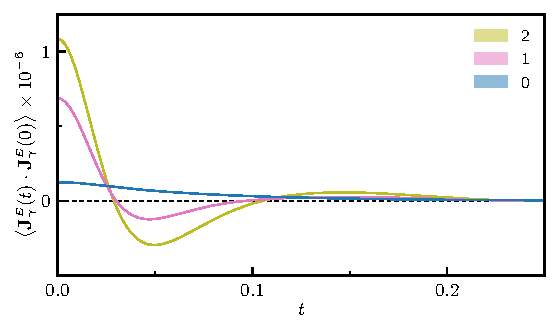
\includegraphics[width=10cm]{chapters/chapter5/figures/handbook_argon_egauge_acf.pdf}}
        \subfigure[\label{fig:kappa-examples}]{****************ESEMPI ARGON - ACQUA - SILICA - MGO ***********} %{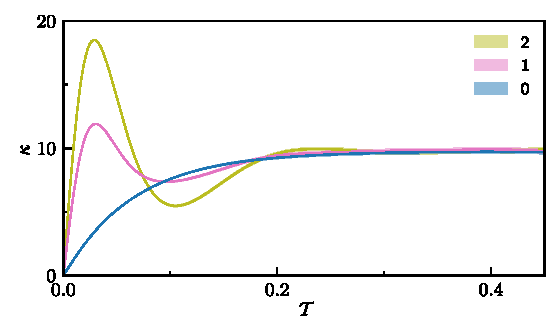
\includegraphics[width=10cm]{chapters/chapter5/figures/handbook_argon_egauge_kappa.pdf}}
    \end{center}
	\caption{(a) Time correlation function of the energy current, Eq.~\eqref{eq:JtJ0}, and (b) the thermal conductivity as a function of the upper limit of integration, Eqs.~(\ref{eq:Lij-integralT}-\ref{eq:kappa-integralT}), computed from MD trajectories for Ar, H$_2$O, MgO, and a-SiO$_2$,
	The green and red lines are computed from two different $100\un{ps}$ trajectories; the blue line is computed from a $1\un{ns}$ trajectory.
	The shaded area surrounding each line indicates the error bars, as estimated from standard block analysis.} 
\end{figure}

To illustrate some real examples, we have run classical MD simulations using the \textsc{LAMMPS} package \cite{LAMMPS1995} of four paradigmatic systems representative of different classes of materials, with the following setup:
\begin{itemize}
    \item \textbf{liquid Ar}: Lennard-Jones potential as described in Ref.~\cite{Argon-FF}, at a temperature $T\approx 220\un{K}$ and density $\rho=1.55\un{g/cm^3}$, in a cubic supercell containing 864 atoms, with a time step $\Delta t=4\un{fs}$.
    \item \textbf{liquid H$_2$O}: Flexible model as in Ref.~\cite{Water-FF} at a temperature $T\approx 300\un{K}$ and density $\rho=1.0\un{g/cm^3}$, in a cubic supercell containing 180 molecules, with a time step $\Delta t=0.5\un{fs}$.
    \item \textbf{crystalline fcc MgO}: Buckingham-plus-Coulomb potential as in Ref. \cite{MgO-FF} at a temperature $T\approx 1000\un{K}$ and density $\rho=3.61\un{g/cm^3}$, in a $4\times 4\times 4$ simple cubic conventional supercell with 512 atoms, and a time step $\Delta t=0.3\un{fs}$
    \item \textbf{amorphous SiO$_2$}: BKS potential \cite{Silica-BKS-1990} as implemented by \citet{Mantisi2012} (see Sec.~\ref{sec:results-class}) at a temperature $T\approx 1000\un{K}$ and density $\rho=2.29\un{g/cm^3}$,  in a supercell containing 216 atoms with a time step $\Delta t=1\un{fs}$. The glass model was obtained from a quench from the melt ($T\approx 6500\un{K}$) at a constant quenching rate of $5.5\times 10^{12}\un{K/s}$.
\end{itemize}
Each system was equilibrated in the NVT ensemble at the target temperature for several hundred picoseconds; data were then collected in the NVE ensemble and analyzed. 
We will also use these systems to benchmark the cepstral analysis method presented in Sec.~\ref{sec:cepstral-analysis}. 

The HCACFs computed for these materials are shown in Fig.~\ref{fig:acf-examples}. 
Liquid argon's HCACF is characterized by a simple exponential decay, characteristic of a simple diffusing liquid. The HCACFs of the other systems, instead, are characterized by an initial drop, followed by a much longer tail, with fast superimposed oscillations caused by the fast intramolecular vibrations (they can thought to be linked to the optical phonon modes of the system). MgO, being a crystalline solid, exhibits the longest correlations, due to the long lifetimes of its propagating phonons. Water and silica, instead, have similar HCACFs, that decay quite fast but feature high-frequency oscillations that persist at long time-lags.

When a HCACF is computed from a trajectory of finite length $\mathcal{T}$, the statistical error increases with the time-lag $t$, as larger time-lags have less statistics. In Fig.~\ref{fig:acf-examples} three examples of HCACFs are plotted: two of them are computed from a $100\un{ps}$ trajectory and present more oscillations and a larger statistical error with respect to the the third HCACF, that is computed from a $1\un{ns}$ trajectory and shows a smoother decay.


\subsection{Direct integration}  \label{sec:direct-integration}
The evaluation of the GK integral, Eq.~\eqref{eq:GK}, or more generally of an Onsager coefficient $L^{ij}$, Eq.~\eqref{eq:L_def}, can simply be performed by direct integration of Eq.~\eqref{eq:JtJ0} as a function of the upper limit of integration: 
\begin{equation}
    L^{ij}(\mathtt{T}) = \frac{\rOmega}{k_B} \int_0^{\mathtt{T}} \langle J^i(t)J^j(0)\rangle \,dt ,  \label{eq:Lij-integralT}
\end{equation}
with $\mathtt{T} < \mathcal{T}$. 
One then recovers, via Eq.~\eqref{eq:multi_kappa}, an estimate for the thermal conductivity dependent on $\mathtt{T}$:
\begin{equation}
    \kappa(\mathtt{T}) = \frac{1}{T^2} \frac{1}{(L^{-1}(\mathtt{T}))^{\smallone\smallone}}.  \label{eq:kappa-integralT}
\end{equation}
This function is usually very noisy: in fact, at times greater than the correlation time between $J^i$ and $J^j$, the correlation function $\langle J^i(t)J^j(0)\rangle$ approaches zero, hence $L^{ij}(\mathtt{T})$ starts integrating pure noise and behaves like the distance traveled by a random walk, whose variance grows linearly with the upper integration limit, as can be appreciated in Fig.~\ref{fig:kappa-examples}.
The evaluation of transport coefficients thus requires averaging over multiple trajectories (possibly multiple segments of a same long trajectory) and estimating the resulting uncertainty as a function of both the length of each trajectory and the upper limit of integration, usually with standard \emph{block analysis} \cite{Frenkel2001}. This is a cumbersome task that often leads to a poor estimate of the statistical and systematic errors on the computed conductivity. All the more so when the signal is inherently oscillatory, due to the existence of high-frequency features, possibly due to intramolecular oscillations that meddle with the noise and can make the convergence of the GK not obvious.

The accuracy of the transport coefficient $\kappa$ estimated by a direct integration of Eq.~\eqref{eq:Lij-integralT} is subject to three possible sources of errors:
\begin{itemize}
    \item[-] \emph{averaging error}: the finite simulation length $\mathcal{T}$ over which the HCACF is computed, Eq.~\eqref{eq:JtJ0}.
    \item[-] \emph{truncation error}: the upper limit of integration $\mathtt{T}$ used in the estimation of $L^{ij}$, Eq.~\eqref{eq:Lij-integralT}, that should be much greater than the characteristic decay time of the correlation.
    \item[-] \emph{discretization/aliasing error}: the finite sampling interval of the heat current, $\epsilon$, that should be large enough to avoid aliasing effects. The Nyqvist-Shannon sampling theorem \cite{Oppenheim1999} states that the sampling period should be smaller than $\frac{1}{2f_\mathrm{max}}$, where $f_\mathrm{max}$ is the maximum frequency of the heat flux signal $J(t)$.
\end{itemize}
Studying the HCACF directly is very difficult, due to the fact that its values are correlated close time-lags. 
If the fluctuations of $J(t)$ follow a Gaussian process, the variance of the HCACF estimated from a finite simulation time $\mathcal{T}$, that we denote with $\mathcal{C}_\mathcal{T}(t)$, tends to the following limits \cite{Jones2012}:
\begin{equation}
    \mathrm{var} \left(\mathcal{C}_\mathcal{T}(t)\right) \sim \left\{
    \begin{aligned}
        4 \frac{\tilde\tau}{\mathcal{T}} \langle \mathcal{C}_\mathcal{T}(0) \rangle^2 , \quad &\text{for }t\rightarrow 0 , \\
        2 \frac{\tilde\tau}{\mathcal{T}} \langle \mathcal{C}_\mathcal{T}(0) \rangle^2 , \quad &\text{for }t\rightarrow \infty ,
    \end{aligned} \right.
\end{equation}
where $\tilde\tau = \frac{\int_0^\infty \langle \mathcal{C}_\mathcal{T}(t) \rangle^2 dt}{\langle \mathcal{C}_\mathcal{T}(0) \rangle^2}$. The variance of the transport coefficient estimator computed from Eq.~\eqref{eq:Lij-integralT} with a cutoff $\mathtt{T}$ thus satisfies the relation:
\begin{equation}
    \mathrm{var} \left(L^{ij}(\mathtt{T})\right) < 4 \left(L^{ij}\right)^2 \frac{\mathtt{T}}{\mathcal{T}} ,
\end{equation}
where $L^{ij}$ is the true transport coefficient, that is valid when $\mathtt{T}$ and $\mathcal{T}$ are much larger than the characteristic decay of the correlation \cite{Jones2012}.

\begin{figure}[!tb]
    \begin{center}
        \subfigure[\label{fig:argon-gk-phases-acf}]{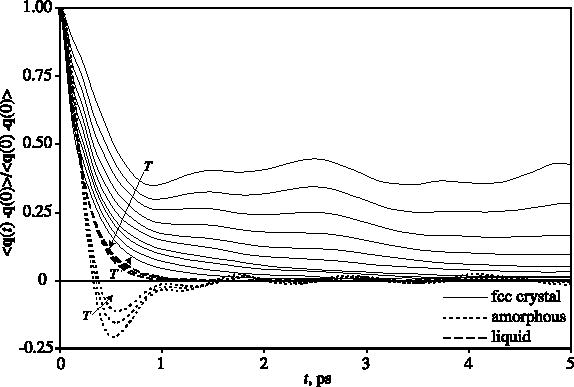
\includegraphics[height=4.5cm]{chapters/chapter5/figures/McGaughey-argon-acf.pdf}}
        \hfill
        \subfigure[\label{fig:argon-gk-phases-kappa}]{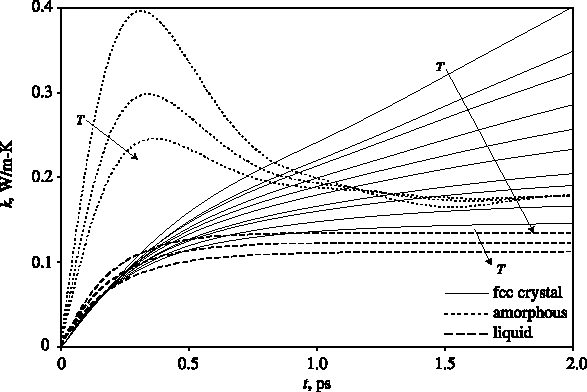
\includegraphics[height=4.5cm]{chapters/chapter5/figures/McGaughey-argon-kappa.pdf}}
    \end{center}
	\caption{(a) Heat current autocorrelation function, Eq.~\eqref{eq:JtJ0}, and
    (b) thermal conductivity as a function of the upper integration limit, Eqs.~(\ref{eq:Lij-integralT}-\ref{eq:kappa-integralT}), for three phases of LJ argon. Reproduced from Ref.~\cite{McGaughey2004a}.} \label{fig:argon-gk-phases-examples}
\end{figure}
\citet{McGaughey2006,McGaughey2004a} studied the thermal conductivity of LJ argon in different phases: fcc crystal, liquid, and amorphous. In Fig.~\ref{fig:argon-gk-phases-examples} we report the comparisons of the HCACFs of these three phases and their direct GK integrals, Eq.~\eqref{eq:kappa-integralT}. At finite time the HCACFs of solid Ar show the two-stage decay \cite{Ladd1986}, and their extension decreases as the temperature increases, as one would expect due to the decrease of phonons relaxation times. 
Their integral converges to the correspondent value of thermal conductivity, however the practical determination of $\kappa$ may be quite subjective. Actually, in the majority of the GK studies reported in the literature, the criteria used to choose an upper limit of integration is not specified, so we guess that they are often based on simple assumption of convergence ``by sight''. 
A few exceptions are listed in the following. For example, the ``first dip'' (FD) method, proposed by \citet{Li1998}, specifies the upper limit of integration by setting the upper limit of integration to be the first time at which the HCACF goes negative. FD may give acceptable results in solid and liquid argon, but it is not suitable to the amorphous phase and in systems with multi-atom unit cell, where the HCACF oscillates wildly around zero before slowly fading out. 

In the case of unit cells with multiple atoms, where intramolecular vibrations manifest as fast oscillations in the HCACF, again, the EF method is not suited to determine $\kappa$. A rather arbitrary compromise was used by \citet{McGaughey2004b}: the GK integral function, Eq.~\eqref{eq:Lij-integralT}, is filtered with a running average \cite{MovingAverage} and the value at which it looks to converge is chosen. If the convergence is not clear one chooses to stop the integration at the point at which the oscillations of $L^{ij}(\mathtt{T})$ reach a minimum (neck). 

Other methods to to perform error analysis have been devised, based on either heuristic or rigorous arguments \cite{Howell2012,Chen2010,Jones2012,Wang_gk2017,Oliveira2017}. All require an estimate of an optimal value for the upper limit of integration, which determines a bias in the estimate, and which is in general difficult to obtain. Moreover most of them are specifically conceived and tested on crystalline solids, such as silicon, and are not suited to study disordered and complex systems. 
For example, \citet{Jones2012} proposed a heuristic on-the-fly algorithm to detect the convergence of the block average of $\kappa$, but that needs an empirical estimate of the maximum correlation time first, and thus it is not optimal. A similar empirical criterion has also been proposed by \citet{Wang_gk2017}. \citet{Oliveira2017}, instead, proposed a method that analyses the components of the noise of the GK integral and fits them with integral functions, in order to obtain an estimate of the uncertainty on $\kappa$ of graphite. 


\subsection{Exponential fit and thermal conductivity decomposition}  \label{sec:exp-fit-decomposition}
Another technique proposed by some authors is the exponential fit (EF) method, in which a single or multi-exponential function is fitted to the HCACF beyond a certain point (determined on a case-by-case basis) \cite{Che2000a,Li1998,Zhang2015}. An example is the function \cite{Che2000a}:
\begin{equation}
    \langle J(t) J(0) \rangle = A_{\mathrm{ac,sh}} \mathrm{e}^{-t/\tau_{\mathrm{ac,sh}}} + A_{\mathrm{ac,lg}} \mathrm{e}^{-t/\tau_{\mathrm{ac,lg}}},
\end{equation}
where the subscripts ``$\mathrm{ac,sh}$'' and ``$\mathrm{lg}$'' refer to acoustic, short-, and long range. From here the thermal conductivity is then estimated as:
\begin{equation}
    \kappa = \frac{\rOmega}{k_B T^2} (A_{\mathrm{ac,sh}}\tau_{\mathrm{ac,sh}} + A_{\mathrm{ac,lg}}\tau_{\mathrm{ac,lg}})  =  \kappa_{\mathrm{ac,sh}} + \kappa_{\mathrm{ac,lg}}. \label{eq:kappa-2exp-fit}
\end{equation}
\citet{McGaughey2004a} interpreted the two-stage behavior of solid argon's HCACF and the resulting decomposition of the thermal conductivity in the context of the mean phonon relaxation time: $\kappa_{\mathrm{ac,sh}}$ corresponds to the phonons with lowest relaxation times,\footnote{\emph{i.e.} phonons with a mean free path equal to one half of its wavelength, the shortest possible. This is also called the CP limit, a thermal conductivity model developed for amorphous materials \cite{Cahill1989,Cahill1992}.} whereas $\kappa_{\mathrm{ac,lg}}$ corresponds to phonons with longer relaxation times, that make the longer decay time of the HCACF.
This model works fairly well \emph{e.g.} for solid argon \cite{McGaughey2004a}, diamond and carbon nanotubes \cite{Che2000a,Che2000b}, as well as in liquid argon, where a single-exponential decay is found, but does not work well to fit the long tails of the HCACF of silicon \cite{Schelling2002}.

The HCACF of amorphous argon, though, shows a different behavior with respect to the solid an liquid phases. It is very similar to the velocity autocorrelation function and can be interpreted considering the different local environments the atoms experience. In a crystal each atom is immersed in the same local environment and the same is true in a liquid, if we average over time. Conversely, in an amorphous solid each atom has a different local environment: close to its equilibrium position, it experiences the free trajectory of a liquid atom at short time scales; but at slightly larger times it feels the interactions of the other atoms, that change its trajectory, and make the correlation negative. 
The first timescale of the HCACF decomposition, $\tau_{\mathrm{ac,sh}}$, is related to the time it takes for the energy to move between nearest-neighbor atoms, and corresponds to the higher frequencies of the acoustic branches. The $\kappa_{\mathrm{ac,sh}}$ is the only one important in the liquid and amorphous phase, it is a function of the coordination of the atoms and scarcely depends on temperature, whereas $\kappa_{\mathrm{ac,lg}}$ strongly depends on temperature.

When fast oscillations of the HCACF are present, such as in multi-atom unit cells, \citet{McGaughey2004b} attempted to fit the filtered HCACF with Eq.~\eqref{eq:kappa-2exp-fit} plus a sum of oscillating terms, that they associated to the ``optical'' modes of the system. 
%A more advanced fit can be performed in this case using the form \cite{McGaughey2004b}:
%\begin{multline}
%    \langle J(t) J(0) \rangle = A_{\mathrm{ac,sh}} \mathrm{e}^{-t/\tau_{\mathrm{ac,sh}}} + A_{\mathrm{ac,lg}} \mathrm{e}^{-t/\tau_{\mathrm{ac,lg}}} \\
%        + \sum_i B_{\mathrm{op},i} \mathrm{e}^{-t/\tau_{\mathrm{op},i}} \cos(\omega_{\mathrm{op},i},t),
%\end{multline}
%\begin{equation}
%    \begin{aligned}
%        \kappa &= \frac{\rOmega}{k_B T^2} \left(A_{\mathrm{ac,sh}}\tau_{\mathrm{ac,sh}} + A_{\mathrm{ac,lg}}\tau_{\mathrm{ac,lg}} + \sum_i \frac{B_{\mathrm{op},i}\tau_{\mathrm{op},i}}{1+\tau_{\mathrm{op},i}^2\omega_{\mathrm{op},i}^2}\right) \\
%        &= \kappa_{\mathrm{ac,sh}} + \kappa_{acf,lg} + \kappa_{\mathrm{op}},
%    \end{aligned}
%\end{equation}
%where the subscript ``$\mathrm{op}$'' refers to optical phonon modes. 
Nevertheless, this fitting procedure is very difficult and it was found to be unsuitable for materials like amorphous silica, that therefore requires either a direct integration or an alternative approach.


\subsection{Spectral methods}  \label{sec:spectral-methods}
\begin{figure}[!tb]
    \begin{center}
        \subfigure[\label{fig:aSi-expfit}]{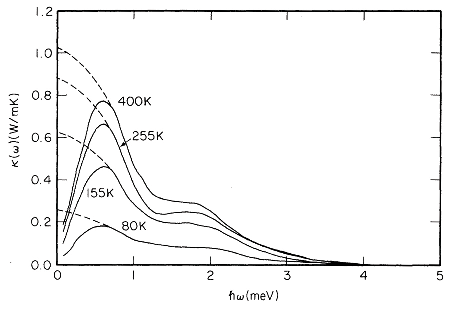
\includegraphics[height=5cm]{chapters/chapter5/figures/Lee-aSi-fit.pdf}}
        \hfill
        \subfigure[\label{fig:cSi-expfit}]{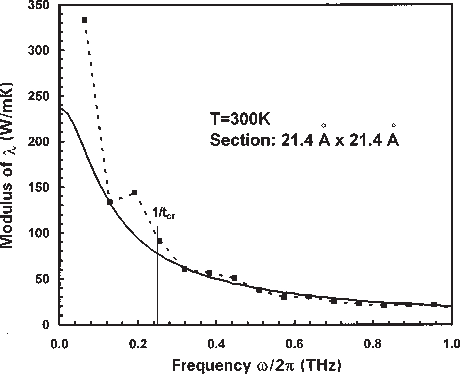
\includegraphics[height=5cm]{chapters/chapter5/figures/Volz-cSi-fit.pdf}}
    \end{center}
	\caption{
	(a) Power spectrum of the heat current of amorphous silicon (solid lines) and the extrapolation required to obtain $\kappa$ (dashed lines). Reproduced from Ref.~\cite{Lee1991}. 
	(b) Power spectrum of the heat current of crystalline silicon (dashed line) and extrapolation required to obtain $\kappa$ (solid line). $t_\mathrm{cr}$ is an estimate of the time required for phonons to propagate across the simulation domain ballistically: \citet{Volz2000} argue that for frequencies lower than this mark, phonons will be affected by artificial correlations due to the finite size of the cell. Reproduced from Ref.~\cite{Volz2000}. 
	} \label{fig:psd-expfit-examples}
\end{figure}
As was shown in Sec.~\ref{sec:Einstein}, the Wiener-Khintchine theorem allows one to express the heat conductivity in terms of the zero-frequency value of the power spectrum of the energy-flux (see Eqs.~(\ref{eq:Wiener-Khintchine}-\ref{eq:GK-S0})):
\begin{equation}
    \kappa = \frac{\rOmega}{2k_B T^2} S (\omega=0). \label{eq:kappa-S0}
\end{equation}
Extrapolating this limit can be very difficult if the statistical properties of the power spectrum are not taken properly into account, as we will argument in Sec.~\ref{sec:cepstral-analysis}.

Some attempts were made to estimate the thermal conductivity by extrapolating the low-frequency region of the spectrum with one Lorentzian function (see Fig.~\ref{fig:psd-expfit-examples}) \cite{Lee1991,Volz2000}.
% (or two Lorentzian function, \emph{e.g.} \cite{Hirosaki2002}:
%\begin{equation}
%    S(\omega) = \frac{1}{\mathcal{T}} \left(\frac{A_1\tau_1}{\sqrt{1+\omega^2\tau_1^2}} + \frac{A_2\tau_2}{\sqrt{1+\omega^2\tau_2^2}} \right) ,
%\end{equation}
%or more simply with $A_2=0$ \cite{Lee1991,Volz2000}. 
This is the Fourier transform of an exponential correlation function, hence, not suprisingly, this expression is in good agreement with time integration results when the HCACF is well modeled by one exponential, but does not work when a long tail is present in the HCACF and whenever the exponential fit is inappropriate \cite{Schelling2002}. The same applies if we consider the sum of two Lorentzians, \emph{i.e.} the sum of two exponential functions in the time domain \cite{Hirosaki2002}. 

The rationale behind these fits given by \citet{Lee1991} and \cite{Volz2000} were finite-size effects. 
The finite size of the simulation cell sets a lower limit to the phonon wavelength that is allowed. Only phonons with a wavelength shorter than the cell size are permitted to exist in the simulation domain and can contribute to the thermal conductivity.
Furthermore, the small cell size may introduce artificial autocorrelations that do not exist in real systems, an effect that will be especially strong for long-wavelength phonons with long mean-free paths. 
\citet{Lee1991} attributed the dip in the heat-current power spectrum of amorphous silicon found at low-frequencies (shown in Fig.~\ref{fig:aSi-expfit}) to this phenomenon, while \citet{Volz2000} attributed it to the apparent divergence of the heat-current power spectrum of crystalline silicon, reported in Fig.~\ref{fig:cSi-expfit}.
\LEnote{**?In our experience, the power spectrum of amorphous silicon does have a shape similar to Fig.~\ref{fig:aSi-expfit}, with a dip at low-frequencies that however does not vanish even when considering much larger sized. ****FIGURA????******}

It is not easy to determine \emph{a priori} at what level the power spectrum is affected by finite-size effects. In any case, let us notice that the size-dependence problem in the estimation of $\kappa$ is also present in other methods, such as the direct integration of the GK equation. In general, one should be careful to verify that the chosen simulation cell is big enough for the thermal conductivity to converge. This will also imply that low-frequency region of the power spectrum is correctly reproduced and does not exhibit unphysical features. We will come back on this issue in Ch.~\ref{ch:silica}. 
In Sec.~\ref{sec:cepstral-analysis} we will start from Eq.~\eqref{eq:kappa-S0} to introduce a more rigorous estimate of the thermal conductivity based on a power spectral analysis, with a solid statistical basis.


\subsection{Estimation from the Einstein relation}
\LEnote{***************}


\subsection{Final remarks}  \label{sec:data-analysis-remarks}

Many methods have been formulated to estimate the thermal conductivity from the GK equation, but none of them is fully satisfactory. Some of them are optimized to the specific case of crystalline solids or simple liquids, and may be a good choice, however they do not really help much when dealing with amorphous solids. 
Different classes of systems require different approaches to error analysis: in some cases these methods fail to provide rigorous criteria to estimate the accuracy resulting from a given MD trajectory, but in general all of them always require very long simulation times, thus making \abinitio simulations unaffordable. 
In Sec.~\ref{sec:cepstral-analysis} we are going to present a novel method that will be able to give an answer to both of these problems, providing us with an efficient and accurate estimator that will allow us to tackle the study of thermal conductivity of disordered systems with equilibrium AIMD simulations. 

In Sec.~\ref{sec:exp-fit-decomposition} we saw that one may try to interpret the decay of HCACF in terms of different relaxation times to get insights into the different contributions to the thermal conductivity, though this is not obvious and clear in general. 
The GK equation is a very general result describing the collective dissipative response of any system to a fluctuation, and it has no intrinsic connection to particular transport mechanisms \cite{Howell2012}. 
The frequencies of the power spectrum of the HCACF have been interpreted to be related to the phonon-phonon interactions \cite{McGaughey2004a}. Conversely, in the BTE approach the thermal conductivity is computed by integrating over the frequencies of individual phonons. The difference between these two frequencies is equivalent to that between the mean free path and the corresponding phonon wavelength. 

However, in the light of the gauge invariance principle presented in Sec.~\ref{ch:gauge-invariance}, at this stage it is not very clear how much the HCACF or the power spectrum of the heat current can be interpreted in physical terms. It is evident that different definitions of the microscopic energy density (or atomic energies) will define different energy currents with very different power spectra, the only invariant quantity being the zero-frequency value, \emph{i.e.} the thermal conductivity. 
\LEnote{**Esempio in Chap 3?**}
Whether and how a particular definition can be linked to physical quantities is not yet completely understood. Therefore, extreme caution should be used when making physical interpretations out of a HCACF. 

In conclusion, although the GK method yields a direct estimate of the thermal conductivity, it provides only very indirect information about the mechanisms of heat transport. We believe that different approaches, such as phonon-level methods, \emph{e.g.} methods based on a normal-modes analysis \cite{Esfarjani2011} may be able to bring better insights into the individual contributions to thermal conductivity, especially in complex or disordered systems. 
\end{LEtext}


%%%%%%%%%%%%%%%%%%%%%%%%%%%%%%%%%%%%%%%%%%%%%%%%%%%%%%%%%%%%%%%%%%%
\section{Cepstral analysis}  \label{sec:cepstral-analysis}

In practice, MD gives access to a discrete sample of the flux process (a \emph{time series}), $J_n = J(n \epsilon)$, $0 \leq n \leq N-1$, where $\epsilon$ is the sampling period of the flux and $N$ the length of the time series, that we assume to be even. 


\subsection{Periodogram}
Let us define the discrete Fourier transform of the flux time series as:
\begin{equation}
  \tilde{J}_{k}=\sum_{n=0}^{N-1} \mathrm{e}^{ 2\pi i\frac{kn}{N}} J_n, \label{eq:Jk}
\end{equation}
for $0 \leq k \leq N-1$.\footnote{Here, the convention for the sign in the exponential of the time-to-frequency Fourier transform is opposite to what adopted in Ref.~\cite{Ercole2017} and in most of the signal analysis literature, in order to comply with the convention for the space-time Fourier transforms usually adopted in the Physics literature and in Eqs.~\eqref{eq:kontinuity} and \eqref{eq:Fourier-continuity}.}
The \emph{sample spectrum} $\hat S_k$, aka \emph{periodogram} in the statistics literature, is defined as
\begin{equation}
\hat{S}_{k}=\frac{\epsilon}{N} \left |\tilde{J}_{k} \right |^2, \label{eq:periodogram-def}
\end{equation}
and, for large $N$, it is an unbiased estimator of the power spectrum of the process, as defined in Eq.~\eqref{eq:Wiener-Khintchine}, evaluated at $\omega_k=2\pi\frac{k}{N\epsilon}$, namely: $\langle \hat S_k \rangle = S(\omega_k)$. The reality of the $\hat J$'s implies that $\tilde J_k=\tilde J^*_{N-k}$ and $\hat S_k=\hat S_{N-k}$, so that periodograms are usually reported for $0\leq k\leq \frac{N}{2}$ and their Fourier transforms evaluated as discrete cosine transforms.

The space autocorrelations of conserved currents are usually short-ranged. Therefore, in the thermodynamic limit the corresponding fluxes can be seen as sums of (almost) independent identically distributed stochastic variables, so that, according to the central-limit theorem, their equilibrium distribution is Gaussian. A slight generalization of this argument allows us to conclude that any conserved-flux process, like the heat flux, is Gaussian as well. The flux time series is in fact a multivariate stochastic variable that, in the thermodynamic limit, results from the sum of (almost) independent variables, thus tending to a multivariate normal deviate. This implies that at equilibrium the real and imaginary parts of the $\tilde J_k$'s defined in Eqs.~\eqref{eq:Jk} are zero-mean normal deviates that, in the large-$N$ limit, are uncorrelated among themselves and have variances proportional to the power spectrum evaluated at $\omega_k$. For $k=0$ or $k=\frac{N}{2}$, $\tilde J_k$ is real and $\sim \mathcal{N}\left (0, \frac{N}{\epsilon}S(\omega_k) \right )$; for $k\notin\left\{ 0,\frac{N}{2}\right\}$, $\mathfrak{Re}\tilde{J}_k$ and $\mathfrak{Im}\tilde{J}_k$ are independent and both  $\sim \mathcal{N}\left (0, \frac{N}{2 \epsilon}S(\omega_k) \right )$, where $\mathcal{N} (\mu,\sigma^2)$ indicates a normal deviate with mean $\mu$ and variance $\sigma^2$. We conclude that in the large-$N$ limit the sample spectrum of the heat-flux time series reads:
\begin{equation}
\hat{S}_{k} = S(\omega_k) \,\xi_{k} \,, \label{eq:periodogram-distribution}
\end{equation}
where the $ {\xi}$'s are independent random variables distributed as a $\chi_1^2$ variate for $k=0$ or $k=\frac{N}{2}$ and as one half a $\chi_2^2$ variate, otherwise. Here and in the following $\chi^2_\nu$ indicates the chi-square distribution with $\nu$ degrees of freedom. For the sake of simplicity, we make as though all the ${\xi}$'s were identically distributed as $\xi_k \sim \frac{1}{2} \chi_2^2$ for all values of $k$, thus making an error of order $\mathcal{O}(1/N)$, which vanishes in the long-time limit that is being assumed throughout this section.


\paragraph{Multiple samples}
In many cases of practical interest, multiple time series are available to estimate the power spectrum of a same process, $\{^{p\!}J_n\}$, $p=1, \cdots \ell$. For instance, in equilibrium MD a same trajectory delivers one independent time series per Cartesian component of the heat flux, all of which are obviously equivalent in isotropic systems. In these cases it is expedient to define a mean sample spectrum by averaging over the $\ell$ different realizations,
\begin{equation}
    \begin{aligned}
      {^{\ell\!}\hat{S}}_{k}& = \frac{\epsilon}{\ell N} \sum_{p=1}^{\ell}  \left |{^p\!}{\tilde J}_{k} \right |^2 \\
      & = S(\omega_k) {^{\ell\!}{\xi}_{k}} \,,
    \end{aligned}  \label{eq:mean-periodogram}
\end{equation}
where the ${^{\ell\!}\xi}$'s are $\chi_{2\ell}^2$ variates, divided by the number of degrees of freedom:
\begin{equation}
    ^{\ell\!}\xi_{k}\sim\frac{1}{2\ell}\chi_{2\ell}^{2}, \label{eq:chi-square-nu}
\end{equation}
for $k \notin \{ 0,\frac{N}{2} \}$. 

Eqs.~\eqref{eq:periodogram-distribution} and \eqref{eq:mean-periodogram} show that ${^{\ell\!}}{\hat S_0}$ is an unbiased estimator of the zero-frequency value of the power spectrum, $\langle {^{\ell\!}}{\hat S_0} \rangle = S(0)$, and through Eq.~\eqref{eq:kappa-S0}, of the transport coefficients we are after.
However, this estimator is not consistent, \emph{i.e.} its variance does not vanish in the large-$N$ limit. This is so because a longer time series increases the number of discrete frequencies at which the power spectrum is sampled, rather than its accuracy at any one of them.

\begin{figure}[!htb]
    \centering
    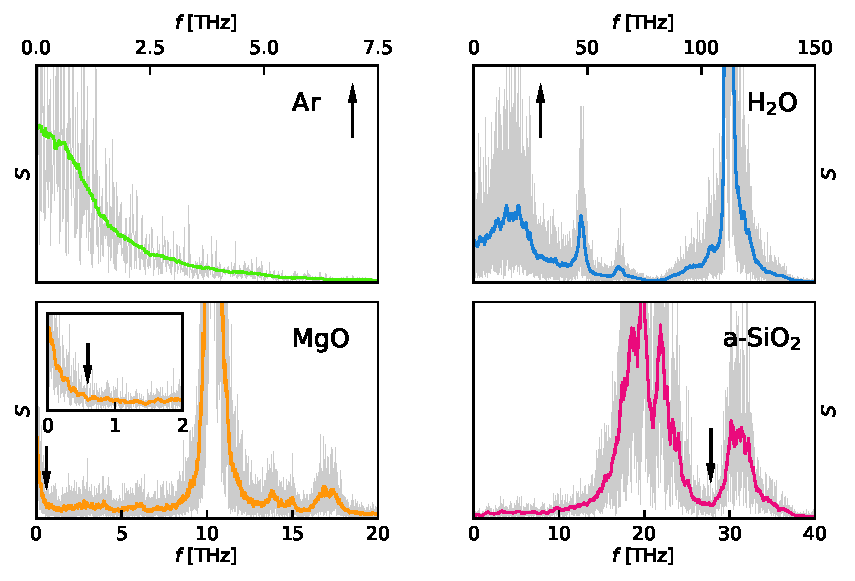
\includegraphics[width=\textwidth]{chapters/chapter5/figures/periodograms.pdf}
    \caption{Sample power spectra of the heat flux computed from MD trajectories for Ar, H$_2$O, a-SiO$_2$ ($100\un{ps}$), and MgO ($500\un{ps}$), obtained directly from Eq.~\eqref{eq:mean-periodogram}, with $\ell=3$ (gray line, see text). The x-axis is frequencies $f=\omega/2\pi$. The solid lines in color correspond to a moving average performed over a narrow frequency window of width $1\un{THz}$, usefult to reveal the main features of the spectrum. The vertical arrows indicate the cutoff frequencies, $f^*$, used for the subsequent cepstral analysis (see text). The inset in the MgO panel is a magnification of the low-frequency region of the spectrum. Reproduced from Ref.~\cite{Ercole2017}.
    }
    \label{fig:periodograms}
\end{figure}

Fig.~\ref{fig:periodograms} displays the periodograms of the heat fluxes of the four systems presented in Sec.~\ref{sec:data-analysis-4systems} (liquid Ar, liquid H$_2$O, crystalline MgO, and amorphous SiO$_2$), obtained from a $100\un{ps}$ ($500\un{ps}$ for MgO) classical MD trajectory in the NVE ensemble and averaged over the three Cartesian components, showing the extremely noisy behavior of the periodogram as an estimator of the spectrum. 
A consistent estimate of the value of the power spectrum at any frequency can be obtained by segmenting a time series into several blocks of equal length and then averaging over the sample spectra computed for each of them. When the length of the trajectory grows large, so does the number of blocks, thus making the variance of the average arbitrarily small. In practice, the determination of the optimal block size is a unwieldy process that leads to an inefficient determination of the length of the trajectory needed to achieve a given overall accuracy. 
Equivalently, a moving average \cite{MovingAverage} of the periodogram would consistently reduce the statistical noise, as happens in Fig.~\ref{fig:periodograms}, but its \emph{multiplicative} nature in Eq.~\eqref{eq:periodogram-distribution} makes it difficult to disentangle the noise from the signal and may introduce a bias. 
Here we adopt a different approach that allows us to obtain a consistent estimate of the zero-frequency value of the power spectrum from the statistical analysis of a \emph{single} trajectory sample (\emph{i.e.} no block analysis is needed) and such that the estimate of the trajectory length necessary to achieve a given accuracy is optimal.

\subsection{Log-periodogram}
Spectral density estimation from finite empirical time series is the subject of a vast literature in the statistical sciences, embracing both parametric and non-parametric methods \cite{Stoica2005}. In the following we propose a semi-parametric method to estimate the power spectrum of a stochastic process, based on a Fourier representation of the logarithm of its power spectrum (the ``log-spectrum''). The advantage of dealing with the log-spectrum, instead of with the power spectrum itself, is twofold. First and foremost, the noise affecting the former is \emph{additive}, instead of multiplicative, thus making it simple and expedient to apply linear filters: limiting the number of components of the Fourier representation of the log-spectrum acts as a low-pass filter that systematically reduces the power of the noise and yields a consistent estimator of the log-spectrum at any given frequency. Second, as a bonus, the logarithm is usually smoother than its argument. Therefore, the Fourier representation of the logarithm of the power spectrum is more parsimonious than that of the spectrum itself.

\begin{figure}
    \centering
    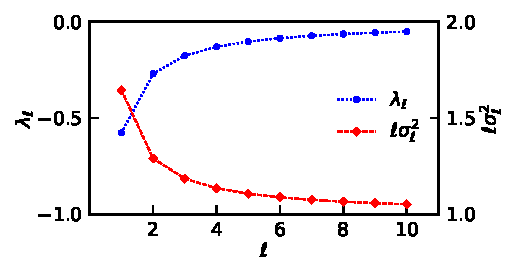
\includegraphics[]{chapters/chapter5/figures/polygamma.pdf}
    \caption{Expectation and variance of the $^{\ell}\lambda$ variables, as defined in Eqs.~(\ref{eq:log-PSD}-\ref{eq:sigma2-ell}), as functions of the number of samples, $\ell$, over which the periodograms are averaged.}
    \label{fig:polygamma}
\end{figure}

Let $^{{\ell\!}}\hat{L}_{k} = \log(^{\ell\!}\hat{S}_{k})$ be the ``\emph{log-periodogram}'' of our time series. By taking the logarithm of Eq.~\eqref{eq:periodogram-distribution}, we can express $^{\ell\!}\hat{L}_{k}$ as:
\begin{align}
    ^{{\ell\!}}\hat{L}_{k} &= \log (^{\ell\!}\hat{S}_{k} ) \nonumber\\
    &= \log\left(S(\omega_k) \right) + \log( ^{\ell\!}{\xi}_k) \nonumber\\
    &= \log\left(S(\omega_k) \right) + {^{\ell\!}\rLambda} + {^{\ell\!}{\lambda}}_{k},  \label{eq:log-PSD}
\end{align}
where
\begin{equation}
    {^{\ell\!}\rLambda} = \left\langle \log( {^{\ell\!}{\xi}}) \right\rangle = \int_0^\infty \log\left (\frac{\xi}{2\ell}\right ) P_{\chi^2_{2\ell}}(\xi) \, d\xi = \psi(\ell)-\log(\ell) \label{eq:lambda-ell}
\end{equation}
is the expected value of the logarithm of the ${^\ell}\hat\xi$ stochastic variables defined in Eq. \eqref{eq:chi-square-nu}, $P_{\chi^2_{2\ell}}$ is the probability density of a $\chi^2_{2\ell}$ variate, $^{\ell\!}{\lambda}_k = \log\left( {^{\ell\!}{\xi}}_k\right) - {^\ell{\rLambda}}$ are zero-mean identically distributed independent stochastic variables, and $\psi(z)$ and is the digamma function \cite{PolyGamma}. 
The variance of the $^{\ell\!}\lambda$ variables is:
\begin{equation}
    \sigma_{\ell}^{2} = \int_0^\infty \log\left (\frac{\xi}{2\ell}\right )^2 P_{\chi^2_{2\ell}}(\xi) \, d\xi - \lambda_{\ell}^2 =\psi'(\ell),\label{eq:sigma2-ell}
\end{equation}
where $\psi'(z)$ is the tri-gamma function \cite{PolyGamma}. 


\subsection{Cepstrum and \emph{lif}tering}

\begin{figure}[!tb]
    \centering
    \LE{**** CEPSTRUMS ****}
    %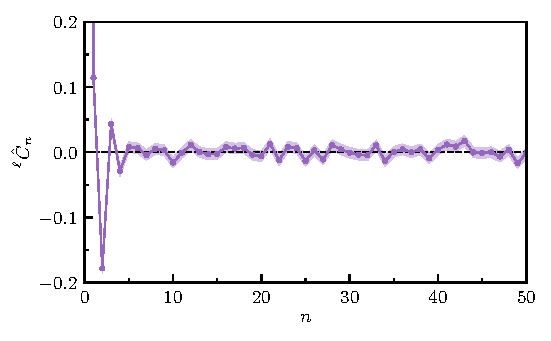
\includegraphics[width=8cm]{chapters/chapter5/figures/handbook_water_cepstrum.pdf}
    \caption{Cepstral coefficients of \LEnote{***...***} computed analyzing the low-frequency region of the periodogram (see Fig.~\ref{fig:periodograms}) and defined in Eq.~\eqref{eq:sample-cepstrum}. }
    \label{fig:cepstrums}
\end{figure}

Eq.~\eqref{eq:log-PSD} explicitly shows that the sample log-spectrum of a time series is equal to the logarithm of the power spectrum one wishes to evaluate (modulo a constant), \emph{plus} a (non-Gaussian) white noise. Whenever the number of (inverse) Fourier components of the logarithm of the power spectrum is much smaller than the length of the time series, applying a low-pass filter to Eq.~\eqref{eq:log-PSD} would result in a reduction of the power of the noise, without affecting the signal. 
In order to exploit this idea, we define the ``\emph{cepstrum}'' of the time series as the inverse Fourier transform of its sample log-spectrum \citep{Childers1977}:
\begin{equation}
  ^{\ell\!} \hat C_{n} = \frac{1}{N}\sum_{k=0}^{N-1} {^{\ell\!} \hat L_{k}} \mathrm{e}^{-2\pi i\frac{kn}{N}}, \label{eq:sample-cepstrum}
\end{equation}
and its coefficients as the \emph{cepstral coefficients} (or ``\emph{que}frencies''). 
A generalized central-limit theorem for Fourier transforms of stationary time series ensures that, in the large-$N$ limit, these coefficients are a set of independent (almost) identically distributed zero-mean normal deviates \citep{Anderson1994,Peligrad2010}. It follows that:
\begin{align}
    ^{\ell\!} \hat  C_{n} &= \lambda_{\ell} \delta_{n0} + C_{n} +  {^{{\ell\!}}{\mu}}_{n},  \label{eq:cepstrogram}\\
    C_{n} &= \frac{1}{N}\sum_{k=0}^{N-1} \log\bigl (S(\omega_k) \bigr ) \mathrm{e}^{-2\pi i\frac{kn}{N}}, \label{eq:C-nohat}
\end{align}
where $^{{\ell\!}}{\mu}_{n}$ are independent zero-mean \emph{normal} deviates with variances $\left\langle {^{{\ell\!}}{\mu}_{n}^2}  \right\rangle$ $=\frac{1}{N}\sigma_\ell^2$ for $n\notin\left\{ 0,\frac{N}{2}\right\}$ and $\left\langle ^{{\ell\!}}{\mu}_{n}^{2}\right\rangle =\frac{2}{N}\sigma_{\ell}^{2}$
otherwise.
This result can be easily checked explicitly by using the definition of the discrete Fourier transform; the non-trivial extra information provided by the central-limit theorem is the asymptotic independence and normality of the $^{\ell}\mu$'s. Similarly to the sample power spectrum, the cepstral coefficients are real, periodic, and even: $\hat C_{n} = \hat C_{N-n}$. 
\begin{LEtext}
In some sense, the cepstrum can be interpreted as a sort of correlation function in a pseudo-time domain. However, it differentiates from the original HCACF for the fact its coefficients are mutually independent and normally distributed, whereas the HCACF values at close time-lags are correlated. 
The word ``cepstrum'' was coined to distinguish it from the spectrum of a signal, and its coefficients essentially give information about the rate of change in the different spectrum bands. This concept has found many applications in voice recognition, pitch detection, characterization of seismic and radar echoes, and more. 
\end{LEtext}


\paragraph{A thermal conductivity estimator}
If the log-spectrum, $\log(S(f_k))$, is smooth enough, the number of non-negligible $C_n$ coefficients in Eq. \eqref{eq:C-nohat} is much smaller than $N$. 
For example, Fig.~\ref{fig:cepstrums} displays the cepstral coefficients of the low-frequency region of the spectrum of the four systems (marked in Fig.~\ref{fig:periodograms}), showing that only the first few coefficients are substantially different from zero. 
Therefore, let us indicate by $P^*$ the smallest integer such that $C_n \approx 0$ for $P^* \le n \le N-P^*$. By limiting the Fourier transform of the sample cepstrum, Eq.~\eqref{eq:sample-cepstrum}, to $P^*$ coefficients, we obtain an efficient estimator of the zero-frequency component of the log-spectrum as:
\begin{equation}
  \begin{aligned}
    ^{\ell\!}\hat{L}_{0}^{*} & = {^{\ell\!}\hat{C}}_{0} + 2 \sum_{n=1}^{P^{*}-1} {^{\ell\!}\hat{C}}_{n} \\
    & = {^{\ell\!}\rLambda} + \log(S_0) + {^{\ell\!} \mu_{0}} + 2 \sum_{n=1}^{P^*-1} {^{\ell\!}} \mu_{n} \,.
  \end{aligned} \label{eq:L0*}
\end{equation}
Inspection of Eq.~\eqref{eq:L0*} shows that $^{\ell\!}\hat{L}_{0}^{*}$ is a normal estimator whose expectation and variance are:
\begin{align}
	\langle {^{\ell\!}}\hat{L}_{0}^{*} \rangle &= \log(S_{0}) + {^{\ell\!}}\rLambda \,, \label{eq:L*} \\
	\sigma_\ell^{*}(P^{*},N)^{2} &= \frac{4P^{*}-2}{N} \sigma_{\ell}^{2} \,. \label{eq:sigma*}
\end{align}
Using Eq.~\eqref{eq:kappa-S0}, we see that the logarithm of the conductivity can be estimated from the cepstral coefficients of the flux time series through Eqs.~(\ref{eq:L0*}-\ref{eq:sigma*}), and that the resulting estimator is always normal with a variance that depends on the specifc system \emph{only} through the number of these coefficients, $P^*$. Notice that the absolute error on the logarithm of the conductivity directly and nicely yields the relative error on the conductivity itself.
\begin{LEtext}
In a sense, $P^*$ can be interpreted like an upper limit of integration of a correlation function in a pseudo-time domain. Again, the actual differences are the well-behaved statistical properties of the cepstral coefficients, opposed to the HCACF's ones.
\end{LEtext}

The value of $P^{*}$ is a property of the stochastic process underlying the time series, and is therefore independent of $N$: for any given value of $P^{*}$ the variance $\sigma_{\ell}^{*2}$ tends to zero in the large-$N$ limit, and $^\ell\hat{L}^*_0-\rLambda_{\ell}$ is thus a consistent estimator of $\log(S_{0})$. In general, all the cepstral coefficients are different from zero and assuming that many of them actually vanish introduces a bias. 
The efficacy of this approach obviously depends on our ability to estimate the number of coefficients necessary to keep the bias introduced by the truncation to a value smaller than the statistical error (that increases with $P^*$), while maintaining the magnitude of the latter at a prescribed acceptable level. 

The choice of $P^*$ is the subject of \emph{model selection} theory, another vast chapter in the statistical sciences \cite{Claeskens2008}. Among the several tests that have been devised to perform this task, we choose the optimization of the Akaike's information criterion (AIC) \cite{Claeskens2008,Akaike1974}, as described in Sec.~\ref{sec:AIC} below, but other more advanced \emph{model selection} approaches \citep{Claeskens2008} may be more effective.

\begin{figure}[!tb]
    \centering
    %\includegraphics[width=8cm]{chapters/chapter5/figures/filtered_psds.pdf}
    \caption{
    Filtered low-frequency region of the power spectrum of \LEnote{******} obtained by limiting the number of cepstral coefficients to various values of $P^*$, Eq.~\eqref{eq:filtered-psd}. $P^*=7$ is the cutoff value suggested by the Akaike's information criterion, Eq.~\eqref{eq:AIC-P}. Grey: the unfiltered periodogram obtained from Eq.~\eqref{eq:periodogram-def}.
    }  \label{fig:filtered-psds}
\end{figure}
\begin{figure}[!tb]
    \centering
    %\includegraphics[width=8cm]{chapters/chapter5/figures/kappa_convergence.pdf}
    \caption{
    Thermal conductivity of \LEnote{******} estimated from Eqs.~(\ref{eq:L0*}-\ref{eq:sigma*}) as a function of the cutoff, $P^*$. The colored bands indicate one standard deviation as estimated from theory. The vertical dashed line indicates the value suggested by the Akaike's information criterion, Eq.~\eqref{eq:AIC-P}, $P_A^*$.
    }  \label{fig:kappa-convergence-Pstar}
\end{figure}

In Fig.~\ref{fig:filtered-psds} we report the low-frequency region of the spectrum of the four analysed systems obtained by limiting the number of cepstral coefficients to $P^*$:
\begin{equation}
    ^\ell\hat{S}_k^* = \exp\left[ 2\sum_{n=1}^{P^*-1} {}^\ell\hat{C}_n \mathrm{e}^{2\pi i \frac{k n}{N}} + {}^\ell\hat{C}_0 - {}^\ell\rLambda\right], \label{eq:filtered-psd}
\end{equation}
thus showing the filtering effect of this choice.
Finally, Fig.~\ref{fig:kappa-convergence-Pstar} shows the value of thermal conductivities obtained through Eqs.~(\ref{eq:L0*}-\ref{eq:sigma*}).


\begin{LEtext}
\paragraph{Mean of periodograms vs Mean of $L_0$ estimators}
When estimating the value of $L_{0}$ from $\ell$ multiple samples of a same process, one has two options:
\begin{description}
    \item[(a)] compute the mean periodogram ${^{\ell\!}}\hat{S}_k$, Eq.~\eqref{eq:mean-periodogram}, and then compute ${^{\ell\!}}\hat{L}_0^*$ from Eq.~\eqref{eq:L0*}. This leads to Eq.~\eqref{eq:sigma*}:
    \begin{equation}
        \textstyle
        \mathrm{var}\left( {^{\ell\!}}L_0^* \right) = \sigma^*_\ell \left(P^*,N\right)^2 ;
    \end{equation}
    \item[(b)] compute the periodogram of each sample ${^{1\!}}\hat{S}_k$ individually, then weight average the estimator of ${^{1\!}}L_0^*$. This gives
    \begin{equation}
        \textstyle
        \mathrm{var}\left( \frac{1}{\ell} \sum_{i=1}^\ell {^{1\!}}\hat{L}_0^{*i} \right) = \frac{1}{\ell} \sigma_1^* \left(P^*,\frac{N}{\ell}\right)^2 .
    \end{equation}
\end{description}
The ratio of the corresponding variances is $\frac{\sigma_{1}^{2}}{\ell\sigma_{\ell}^{2}} = \frac{\pi^2}{6\ell\psi'(\ell)} > 1$: we conclude that it is more convenient to perform the average over the periodograms (a) instead of on the final estimator (b).

The dependence of $\sigma_{\ell}$ on $\ell$, displayed in Fig.~\ref{fig:polygamma}, gives us a leverage to reduce the variance of the estimate of $L_{0}$, essentially for free. Suppose one partitions each of the $\ell$ time series of $N$ elements into $m$ segments of $N/m$ elements. When the segments are long enough, the sample average evaluated for each of them has the same variance as the value obtained from the entire trajectory, \emph{i.e.} $\sigma_\ell^{*}(P^{*},N/m)^{2}/m = \sigma_\ell^{*}(P^{*},N)^{2}$, thus providing no improvement. If instead one evaluates ${L}_{0}$ from the mean periodogram averaged over the $\ell \times m$ segments, the corresponding variance would be $\sigma_{\ell m}^2(P^*,N/m)$, which is a decreasing function of $m$ (see Fig.~\ref{fig:polygamma}) and tends to $\frac{4P^{*}-2}{\ell N}$ for $\ell m\gg 1$. In practice the asymptotic behavior $\sigma_{\ell}^{2} = \psi'(\ell) \approx 1/\ell$ is reached for $\ell \gtrsim 6$ ($6\sigma_{6}^{2}\approx 1.09$), and we propose to use $m=6$ segments when only one time series is available ($\ell=1$), thus reducing the standard deviation by a factor $\sqrt{\frac{\sigma_{1}^{2}}{6\sigma_{6}^{2}}}\approx 1.23$. When three times series are available, such as in the simulation of thermal transport in isotropic materials ($\ell=3$), the advantage of segmenting the trajectory by choosing \emph{e.g.} $m=2$ segments would be marginal ($\sqrt{\frac{3\sigma_{3}^{2}}{6\sigma_{6}^{2}}} \approx 1.04$), and we choose therefore to keep $m=1$. 
\end{LEtext}


\subsection{Akaike Information Criterion}  \label{sec:AIC}
Given a model depending on $P$ parameters, $\theta = \{\theta_{1}, \theta_{2}, \cdots \theta_{P}\}$, the AIC \cite{Claeskens2008,Akaike1974} is a sample statistic defined as
\begin{equation}
    \mathrm{AIC}(P) =-2\max_{\theta}\log\mathcal{L}(\theta,P)+2P,\label{eq:AIC}
\end{equation}
where $\mathcal{L}(\theta,P)$ is the likelihood of the parameters. The optimal number of parameters is determined as the argument of the AIC minimum:
\begin{equation}
    P_A^* \equiv \arg\min_P\mathrm{AIC}(P) . \label{eq:P*}
\end{equation}

In the present case the parameters of the model are the $P$ coefficients $C=\{C_{0},C_{1},\cdots C_{P-1}\}$ as defined in Eq.~\eqref{eq:C-nohat}, and the log-likelihood reads, up to additive terms independent of $P$ and $C$:
\begin{equation}
    2\log\mathcal{L}(C,P) = -\frac{N}{2\sigma_\ell^{2}}\left(C_{0}+\rLambda_{\ell}-\hat{C}_{0}\right)^{2} -\frac{N}{\sigma_\ell^{2}}\sum_{n=1}^{P-1}\left(C_{n}-\hat{C}_{n}\right)^{2} -\frac{N}{\sigma_\ell^{2}}\sum_{n=P}^{N/2} \hat{C}_{n}^{2} .
\end{equation}
Evidently, the above expression is maximized, for given $P$, by $C_{n} = \hat{C}_{n} - \delta_{n0}\rLambda_{\ell}$ for $n=0,1,\cdots P-1$, and the corresponding value of the maximum is: $2\max_C\log\mathcal{L}(C,P) = -\frac{N}{\sigma_\ell^{2}} \sum_{n=P}^{N/2} \hat{C}_{n}^{2}$.
We conclude that the value of the AIC is:
\begin{equation}
    \mathrm{AIC}(P) = \frac{N}{\sigma_\ell^{2}} \sum_{n=P}^{N/2} \hat{C}_{n}^{2} + 2P . \label{eq:AIC-P}
\end{equation}
The value of $P$ that minimizes this expression is the optimal number of parameters in the Akaike sense, $P_A^*$, as defined in Eq.~\eqref{eq:P*}.
In Fig.~\ref{fig:kappa-convergence-Pstar} the value $P_A^*$ chosen by the AIC for the four systems is indicated.


\subsection{Nyqvist frequency}  \label{sec:cepstral-nyqvist}
The maximum frequency available for spectral/cepstral analysis is the Nyqvist frequency \cite{Oppenheim1999}, determined by the sampling period $\epsilon$ as $f_{\mathrm{Ny}}=\frac{1}{2\epsilon}$ (\emph{i.e.} angular frequency $\omega_{\mathrm{Ny}}=2\pi f_{\mathrm{Ny}}$). Transport coefficients only depend on the low-frequency behavior of the spectrum, which is independent of $\epsilon$, as long as the latter is small enough as to avoid aliasing effects. For this reason it may prove convenient to eliminate the high-frequency portion of the spectrum ($f>f^*$) by applying a low-pass filter to the time series (\emph{e.g.} a moving average \cite{MovingAverage}) and then resample the latter with a sampling period $\epsilon^*=\frac{1}{2f^*}$, thus resulting in a time series of $N^*=N\frac{f^*}{f_{\mathrm{Ny}}}$ time steps.

The optimal number of cepstral coefficients resulting from Eqs.~\eqref{eq:P*} and \eqref{eq:AIC-P}, as well as the error in the estimate of the transport coefficients resulting from Eq.~\eqref{eq:sigma*}, depends in general on the choice of the cutoff frequency, $f^*$. The smaller $f^*$, the smaller will presumably be the number of cepstral coefficients necessary to describe the log-spectrum to any given accuracy over such a shorter frequency range. However, the shorter length of the filtered time series, $N^*$, results in an increased variance of the estimator $^\ell{\hat L^*_0}$ defined in Eq.~\eqref{eq:L0*}, according to Eq.~\eqref{eq:sigma*}. Numerical experiments performed on the MD data reported in Sec.~\ref{sec:cepstral-benchmarks} and Fig.~\ref{fig:kappa_vs_fstar} show that both the estimated value of $^\ell{\hat L^*_0}$ and its variance are actually fairly insensitive to the value chosen for the cutoff frequency, $f^*$, provided that the power spectrum of the re-sampled time series faithfully features the first band of the original spectrum (\emph{i.e.} the first prominent feature) and that this band is not too peaked at the origin.


\subsection{Data analysis work-flow (solids and one-component fluids)}  \label{sec:cepstral-workflow-1comp}
We summarize the steps leading to the estimation of thermal conductivity by the \textit{cepstral analysis} method, in order to highlight the simplicity of its practical implementation.
\begin{enumerate}
    \item From a MD simulation compute the energy flux time series $J_n^i$, $i=1,\cdots\ell$ (usually $\ell=3$ cartesian components).
    \item Compute the discrete Fourier transform of the fluxes, $\tilde{J}_k^i$, and the mean-periodogram $^{\ell\!}\hat{S}_k$ from Eqs.~\eqref{eq:periodogram-def} and \eqref{eq:mean-periodogram}, and smooth it out using \emph{e.g.} a moving average \cite{MovingAverage} performed over a narrow frequency window, so as to reduce the statistical noise to a level where the shape of the power spectrum of the underlying process can be appreciated.\footnote{Mind the difference between the moving average performed in the frequency domain to smooth out the power spectrum and that performed in the time domain, as suggested before, and acting as a low-pass filter. Spectral smoothing using a moving average in the frequency domain is common practice in the analysis of time series, and it actually provides a consistent estimator of the power spectrum. In fact, the number of frequencies falling within a window of given width increases linearly with the length of the series, so that the variance of the average decreases as the inverse of the product of the length of the series times the width of the window. The resulting spectral estimate is however biased by the variation of the signal within the window, thus strongly reducing the width of the windows that can be afforded. Moreover, both the bias and the statistical error are difficult to estimate, due to the multiplicative nature of the noise; therefore neither the plain periodogram nor a running average thereof are adequate for a quantitative estimate of the zero-frequency value of the power spectrum, which is proportional to the transport coefficient we are after.}
    \item Only a selected low-frequency region shall be used in the next steps (see Sec.~\ref{sec:cepstral-nyqvist} and \ref{sec:cepstral-benchmarks} for a detailed discussion): choose a cutoff frequency, $f^*$, so as to encompass the first band of the smoothed power spectrum. 
    \item Compute the log-periodogram ${^{\ell\!}}\hat{L}_k = \log({^{\ell\!}}\hat{S}_k)$.
    \item Compute the inverse discrete Fourier transform of the result to obtain the cepstral coefficients ${^{\ell\!}}\hat{C}_n$, Eq.~\eqref{eq:sample-cepstrum}. 
    \item Apply the Akaike Information Criterion, Eqs.~\eqref{eq:P*} and \eqref{eq:AIC-P}, to estimate the number of cepstral coefficients to retain, $P^*$.
    \item Finally apply Eq.~\eqref{eq:L0*} to obtain ${^{\ell\!}}\hat{L}_0^*$, and evaluate the thermal conductivity as
    \begin{equation}
        \kappa = \frac{\rOmega}{2k_B T^2} \exp\left[\hat{L}_0^* - \psi(\ell) + \log(\ell) \right],
    \end{equation}
    and its statistical error as
    \begin{equation}
        \frac{\rDelta\kappa}{\kappa} = \sqrt{\psi'(\ell) \frac{4P^{*}-2}{N}}.
    \end{equation}
\end{enumerate}


\subsection{Benchmarks}  \label{sec:cepstral-benchmarks}
The cepstral analysis method just presented has been implemented in a Python package, \textsc{ThermoCepstrum} \cite{thermocepstrum}, and benchmarked for the calculation of the thermal conductivity of the four representative systems presented in Sec.~\ref{sec:data-analysis-4systems}: liquid Ar, liquid H$_2$0, crystalline MgO and amorphous SiO$_2$.
After equilibration, data were collected in the NVE ensemble for trajectories whose length was chosen so as to represent realistic simulation runs that could be afforded using \emph{ab initio} MD ($\mathcal{T} = 100\un{ps}$ for Ar, H$_2$O, and a-SiO$_2$, and $\mathcal{T} =500\un{ps}$ for MgO). 
In order to compare our estimates of the transport coefficients and their statistical errors with reliable and statistically significant reference data, in all cases we ran much longer ($\approx 50\un{ns}$) simulations. 
This allowed us to compare our predicted conductivities with accurate values estimated from the direct integration of the GK equation, Eqs.~\eqref{eq:Lij-integralT} and \eqref{eq:kappa-integralT}, as obtained from a block average \cite{Frenkel2001} performed over the long trajectory (see Sec.~\ref{sec:direct-integration}). 
In addition, we could collect abundant statistics of our estimator for the transport coefficients, Eq.~\eqref{eq:L0*}, and validate its normal distribution specified by Eqs.~\eqref{eq:L*} and \eqref{eq:sigma*}. 

The periodograms of one segment of each system are reported in Fig.~\ref{fig:periodograms}, where a moving average in also computed in order to reveal the main features of the power spectrum. 
The values of the cutoff frequencies used for cepstral analysis, $f^*$, are chosen so as to encompass the first prominent feature of the (smoothed) power spectrum. For instance, in H$_2$O and a-SiO$_2$ we choose $f^*\approx 29\un{THz}$ and $f^*\approx 28\un{THz}$, respectively. In MgO we assume $f^*\approx 0.6\un{THz}$, just at the upper edge of the first narrow peak, whereas in Ar there is just one band, corresponding to a purely diffusive behavior of a simple fluid, and we assume $f^*\approx 7\un{THz}$, where the spectrum has exhausted most of the available power, but its value is not yet too small (see Fig.~\ref{fig:periodograms}). The corresponding average numbers of cepstral coefficients given by the optimization of the AIC are: $P_A^*=5$ (Ar), $7$ (H$_2$O), $4$ (MgO), and $31$ (a-SiO$_2$). Later we will display the dependence of the number of optimal cepstral coefficients and of the resulting estimate of the thermal conductivity on the choice of $f^*$, and show that this choice is not critical.

In order to validate our data-analysis protocol, we first computed the heat conductivities from a direct integration of the current autocorrelation function, Eqs.~\eqref{eq:Lij-integralT} and \eqref{eq:kappa-integralT}, combined with standard block analysis over the $50\un{ns}$ long trajectory (see Sec.~\ref{sec:direct-integration}), that will be taken as a reference, obtaining: $\kappa_{\mathrm{ref}} = 0.1965 \pm 0.0015$, $0.970 \pm 0.009$, $19.2 \pm 0.4$, and $2.115 \pm 0.025 \un{W/mK}$, for Ar, H$_2$O, MgO, and a-SiO$_2$, respectively. 
Although our simulations were meant for benchmarking purposes only, and no particular attention was paid to exactly match the simulation conditions of previous work, these data are in fair agreement with the foregoing theoretical results: $\approx 0.19\un{W/mK}$ (Ar) \cite{Argon-FF}, $\approx 0.85\un{W/mK}$ (H$_2$O) \cite{Romer2012}, $\approx 12\un{W/mK}$ (MgO) \cite{MgO-FF}, and $\approx 2.1\un{W/mK}$ (a-SiO$_2$) \cite{Larkin2014}.

\begin{figure}[!tb]
    \centering
    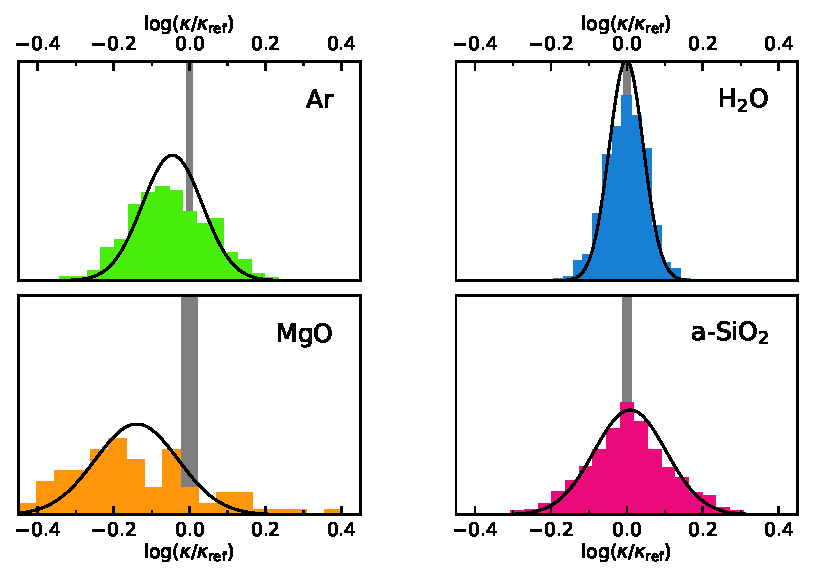
\includegraphics[width=\textwidth]{chapters/chapter5/figures/histograms.pdf}
    \caption{Distributions of the logarithm of the thermal conductivities, $\log(\kappa)$, estimated over multiple MD segments ($100\un{ps}$ for Ar, H$_2$O, and a-SiO$_2$, and $500\un{ps}$ for MgO) extracted from a $50\un{ns}$ long trajectory. The reported data are referred to $\kappa_\mathrm{ref}$, which is the value obtained from a direct integration of the GK equation, combined with standard block analysis over the $50\un{ns}$ trajectory, and represented by the vertical gray bands. The Gaussian curves represent the distributions predicted by the theory, centered at the sample mean. Remember that the absolute error on $\log(\kappa)$ is the relative error on $\kappa$. Reproduced from Ref.~\cite{Ercole2017}.
    }
    \label{fig:histograms}
\end{figure}
\begin{figure}[!tb]
    \centering
    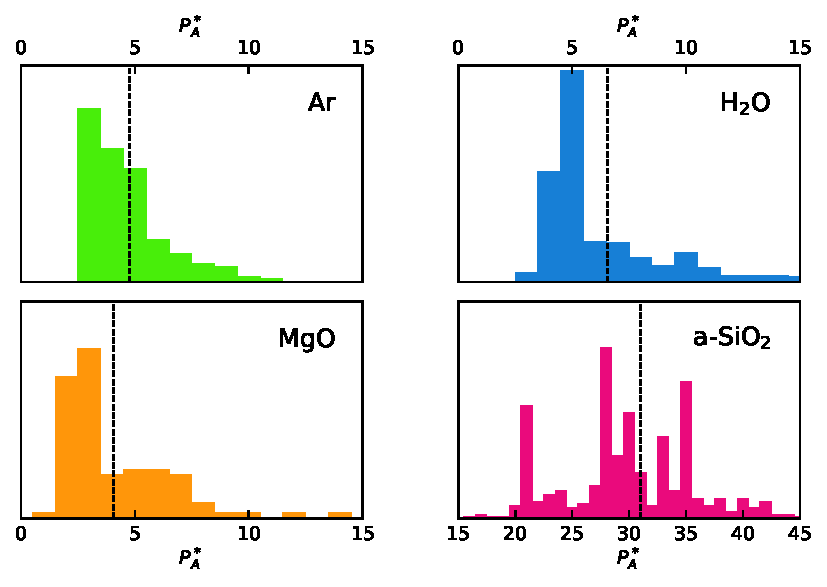
\includegraphics[width=\textwidth]{chapters/chapter5/figures/Pstar_distribution.pdf}
    \caption{Distribution of the optimal numbers of cepstral coefficients, $P_A^*$, as determined by optimizing the Akaike's information criterion, Eqs.~\eqref{eq:P*} and \eqref{eq:AIC-P}, for each segment of the $50\un{ns}$ long MD trajectory, as described in Sec.~\ref{sec:AIC}. The vertical dashed lines indicate the average value of $P_A^*$. Reproduced from Ref.~\cite{Ercole2017}.
    }
    \label{fig:Pstar_distribution}
\end{figure}


\paragraph{Distribution of the estimator of $\kappa$}
In Fig. \ref{fig:histograms} we display the distributions of the values of $\log(\kappa/\kappa_{\mathrm{ref}})$ estimated by applying our protocol to multiple MD segments of $100\un{ps}$ (for Ar, H$_2$O, a-SiO$_2$) and $500\un{ps}$ (for MgO), extracted from the $50\un{ns}$ long trajectory. The optimal numbers of cepstral coefficients, $P^*$, have been redetermined for each segment independently, while the values of the cutoff frequency, $f^*$, which only depends on the qualitative features of the spectrum, have been determined once for all for one of them. The distribution of the resulting number of cepstral coefficients is reported in Fig. \ref{fig:Pstar_distribution}. The observed distributions of $\log(\kappa)$ successfully pass the Shapiro-Wilk normality test \cite{Shapiro1965} (\emph{i.e.} they do not fail it) and the observed sample standard deviations closely match the theoretical values estimated from Eq.~\eqref{eq:sigma*}, as reported in Table~\ref{tab:logkappa-errors}. 
\begin{table}[!htb]
    \centering
    \begin{tabular}{rcc}
                  & \textbf{sample} & \textbf{theory} \\
        \hline
        \textbf{Ar} $(100\un{ps})$       & $0.104$ & $0.079$ \\
        \textbf{H$_2$O} $(100\un{ps})$   & $0.053$ & $0.045$ \\
        \textbf{MgO} $(500\un{ps})$      & $0.17$  & $0.11$ \\
        \textbf{a-SiO$_2$} $(100\un{ps})$ & $0.114$ & $0.095$ \\
    \end{tabular}
    \caption{Observed and theoretical standard deviations of the distributions of $\log(\kappa)$, displayed in Fig.~\ref{fig:histograms}. The theoretical values are obtained from Eq.~\eqref{eq:sigma*}. Remember that the absolute error on $\log(\kappa)$ is the relative error on $\kappa$.}
    \label{tab:logkappa-errors}
\end{table}
Remember that the error on $\log(\kappa)$ is the relative error on $\kappa$: the corresponding absolute errors achievable with a short trajectory of $100$ (Ar, H$_2$O, and a-SiO$_2$) or $500$ (MgO) ps, not to be confused with the long trajectory used to establish the reference data above, are therefore: $\sigma_\kappa \approx 0.015$ (Ar), $0.045$ (H$_2$O), $2$ (MgO), and $0.2$ (a-SiO$_2$) $\mathrm{W/mK}$. This indicates that a \emph{single} and short sample trajectory, such as one that is affordable with \emph{ab initio} MD, is sufficient to achieve and accurately estimate a very decent relative error on the computed transport coefficient. In an attempt to evaluate the thermal conductivity from the direct computation of the GK equation, Eqs.~\eqref{eq:Lij-integralT} and \eqref{eq:kappa-integralT}, and standard block analysis using similarly short MD trajectories, our best estimate of the resulting statistical error was 2-3 times larger than using our protocol (meaning $5-10\times$ longer trajectories to achieve a comparable accuracy) in all cases but liquid Ar, where only a marginal improvement is achieved using our methodology. Much more than this, the standard analysis of MD data depends on a number of hidden parameters, such as the upper limit of the GK integral, Eq.~\eqref{eq:Lij-integralT}, or the width of the blocks for error analysis, that are hard to determine and keep under control, as discussed in Sec.~\ref{sec:direct-integration}. Our method, instead, only depends on a single parameter, the number of cepstral coefficients, whose optimal value can be easily determined from the Akaike's information criterion, or other more sophisticated model-selection methods \cite{Burnham2004,Claeskens2008}, as appropriate.


\paragraph{Bias}
\begin{figure}[!tb]
    \centering
    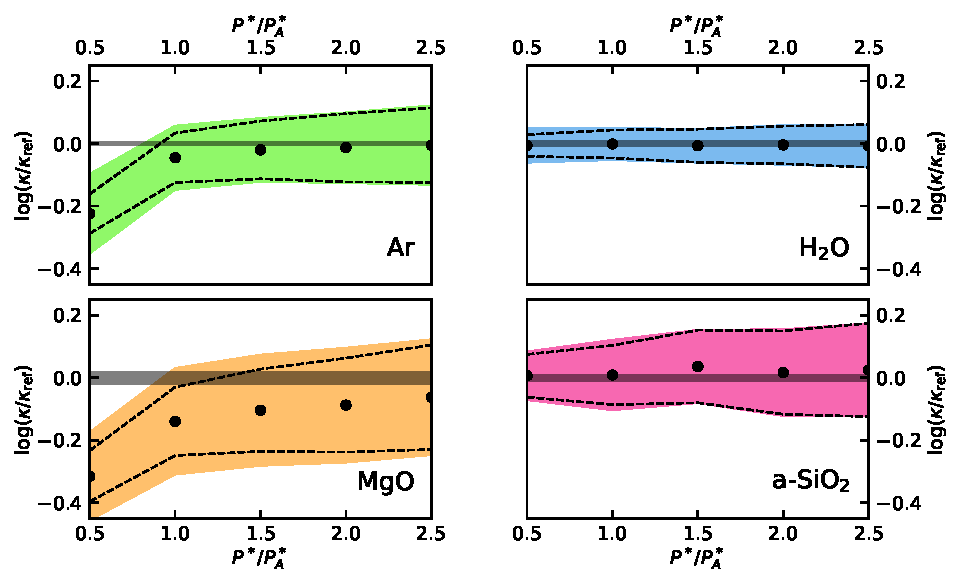
\includegraphics[width=\textwidth]{chapters/chapter5/figures/L-vs-P.pdf}
    \caption{Dependence of $\log(\kappa)$, as estimated from Eq.~\eqref{eq:L0*}, on the number of cepstral coefficients $P^*$. $P_A^*$ is the optimal number of coefficients estimated from the AIC using Eqs.~\eqref{eq:P*} and \eqref{eq:AIC-P}. The black dots represent the mean values of $\log(\kappa)$ computed over multiple MD segments ($100\un{ps}$ for Ar, H$_2$O, and a-SiO$_2$, and $500\un{ps}$ for MgO) extracted from a $50\un{ns}$ long trajectory; the colored bands and dashed lines represent one standard deviation as estimated from the empirical statistics and from Eq.~\eqref{eq:sigma*}, respectively. The reported data are referred to $\kappa_{\mathrm{ref}}$, which is the value of thermal conductivity obtained from a direct integration of the GK equation, combined with standard block analysis over the $50\un{ns}$ trajectory, and represented by the horizontal gray bands. Remember that the absolute error on $\log(\kappa)$ is the relative error on $\kappa$. Reproduced from Ref.~\cite{Ercole2017}.
    }
    \label{fig:L-vs-P}
\end{figure}
\begin{table}[!tb]
    \centering
    \begin{tabular}{ccc}
                  & $\langle\kappa\rangle$ & $\kappa_\mathrm{ref}$ \\
        \hline
        \textbf{Ar}        & $0.1878 \pm 0.0007$ & $0.1965 \pm 0.0015$ \\
        \textbf{H$_2$O}    & $0.969 \pm 0.002$   & $0.970 \pm 0.009$ \\
        \textbf{MgO}       & $16.7 \pm 0.2$      & $19.2 \pm 0.4$ \\
        \textbf{a-SiO$_2$} & $2.131 \pm 0.009$   & $2.115 \pm 0.025$ \\
    \end{tabular}
    \caption{Sample mean of the estimated $\kappa$, computed over the distributions displayed in Fig.~\ref{fig:histograms}; and reference values of thermal conductivity, $\kappa_\mathrm{ref}$, obtained from the direct integration of the GK equation over the $50\un{ns}$ trajectory. Units are $\mathrm{W/mK}$.}
    \label{tab:kappa-bias}
\end{table}
In order to estimate the bias introduced by limiting the number of cepstral coefficients, we examined the sample mean of the estimator of $\kappa$, $\langle\kappa\rangle$, computed over the distributions displayed in Fig.~\ref{fig:histograms}, obtaining the values reported in Table~\ref{tab:kappa-bias}. Comparing these data with the reference data obtained from  the direct evaluation of the GK integral, we see that the bias is negligible for H$_2$O and a-SiO$_2$, very small for Ar, and small but not negligible for MgO. In Fig.~\ref{fig:L-vs-P} we display the dependence of $\log(\kappa/\kappa_{\mathrm{ref}})$ on the number of cepstral coefficients, $P^*$, as estimated from Eq.~\eqref{eq:L0*}. We observe that when the number of cepstral coefficients, $P^*$, is larger than the optimal value determined from the AIC, $P_A^*$, the estimated value of $\kappa$ seems not to depend on $P^*$ for all systems but MgO, for which a slight bias seems to persist, and to a much lesser extent for Ar. Also, Eq.~\eqref{eq:sigma*} seems to slightly underestimate the sample variance for small $P^*$ in these cases. In the case of MgO this behavior is likely due to the difficulty of the AIC to cope with the sharp low-frequency peak in the power spectrum, due to the highly harmonic character and slow decay of the vibrational heat carriers in periodic crystals \cite{Carbogno:2017gc}, thus requiring longer simulation times. In the case of Ar the very small bias observed for $P^* =P^*_A$ may be due to the difficulty of choosing a suitable cutoff frequency when only a single diffusive band is present in the spectrum, and to the divergence of the log-spectrum at high frequency. In all cases, use of the Aikake's information criterion results in a bias that is smaller than the statistical error estimated from an individual short sample trajectory and that can be systematically removed by increasing the value of $P^*$, at the price of increasing the statistical error, if and when needed.


\paragraph{Cutoff frequency $f^*$}
\begin{figure}[!tb]
    \centering
    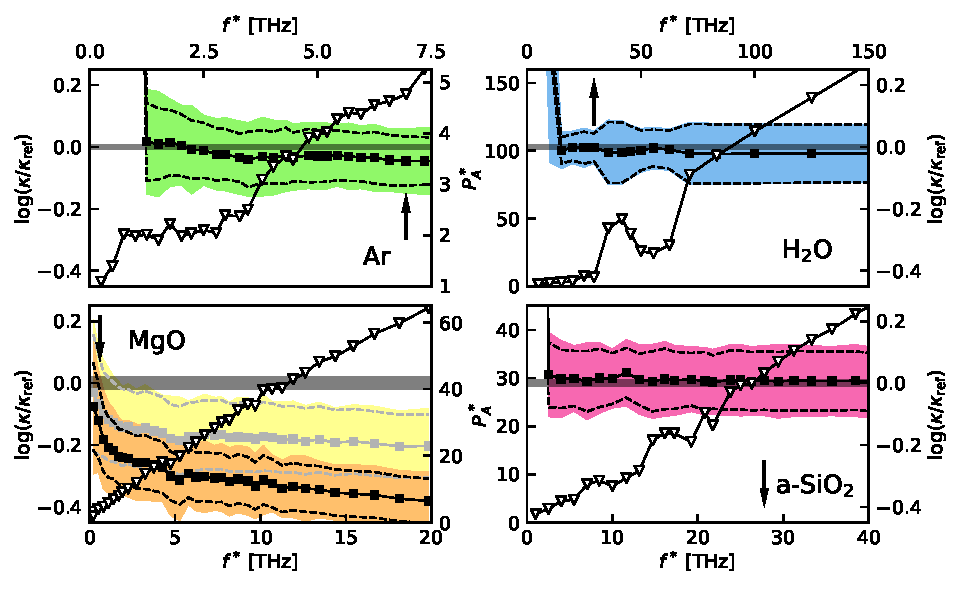
\includegraphics[width=\textwidth]{chapters/chapter5/figures/kappa_vs_fstar.pdf}
    \caption{Triangles: average optimal number of cepstral coefficients, $P_A^*$, as determined by the AIC, Eqs. \eqref{eq:P*} and \eqref{eq:AIC-P}, as a function of the cutoff frequency used for cepstral analysis, $f^*$ (see discussion just after Eq. \eqref{eq:AIC-P}). Squares: $\log(\kappa)$ resulting from a given choice of $f^*$ and of the corresponding value of $P_A^*$. All the values are averages performed over multiple $100\un{ps}$ long segments ($500\un{ps}$ for MgO) extracted from a $50\un{ns}$ long MD trajectory, as discussed in the text. The colored bands indicate the sample standard deviation and the dashed lines that resulting from our theoretical analysis (see Eq. \eqref{eq:sigma*}). The vertical arrows indicate the cutoff frequencies, $f^*$, used for the cepstral analysis in this paper (see Fig. \ref{fig:periodograms} and text). In the case of MgO, the data indicated with lighter colors are obtained using a number of cepstral coefficients twice as large as that provided by the AIC, $P^*=2P_A^*$. The data are referred to $\kappa_{\mathrm{ref}}$, which is the value of thermal conductivity obtained from direct integration of the GK equation over the $50\un{ns}$ trajectory, and represented by the horizontal gray bands. Remember that the absolute error on $\log(\kappa)$ is the relative error on $\kappa$. Reproduced from Ref.~\cite{Ercole2017}.
    }
    \label{fig:kappa_vs_fstar}
\end{figure}
In Fig.~\ref{fig:kappa_vs_fstar} we report the dependence of the optimal number of cepstral coefficients, $P_A^*$, as a function of the cutoff frequency, $f^*$, along with the dependence of the resulting estimate of $\log(\kappa/\kappa_{\mathrm{ref}})$. $P_A^*$ increases (roughly linearly) with $f^*$. Notwithstanding, the estimated value of the heat conductivity, as well as its variance, is fairly insensitive on the precise value of $f^*$ as long as the latter is large enough as to encompass the lowermost prominent feature of the spectrum. 
Some more comments are in order for MgO. In this case the high thermal conductivity, due to the strong harmonic character of slowly decaying phonon modes, manifests in the form of a narrow peak centered at $f=0$, followed by a broad plateau that carries little spectral weight. This feature determines a more pronounced increase in the number of significant cepstral coefficients as $f^*$ increases and a corresponding increase of the bias when keeping $P^*$ at the value given by the AIC. In this case, the AIC is a less reliable indicator of the number of cepstral coefficients necessary to keep the bias low. By increasing this number by a factor of two or more, the bias decreases, as indicated by the results reported in lighter colors in Fig.~\ref{fig:kappa_vs_fstar}, and eventually vanishes, as shown in Fig.~\ref{fig:L-vs-P}.

\begin{LEtext}
\paragraph{Trend with simulation length}
By analyzing the trend of the estimate of $\log(\kappa)$ of MgO with the length of the trajectory segment analyzed, $N$, it appears that by increasing $N$ the bias decreases, and the value of $\log(\kappa)$ becomes less and less dependent on the choice of $f^*$, if we set $P^*=P_A^*$. Not surprisingly, this effect is not present in the other analyzed systems. The number of frequencies of the periodogram used for the cepstral analysis is equal to $N/2$, and the minimum frequency available for analysis is $\Delta f = \frac{1}{N\epsilon}$. 
When the heat flux time series is characterized by a slowly decaying HCACF (a long autocorrelation time) and a sharp peak at $f\approx 0$, like in the case of MgO, a longer trajectory (\emph{i.e.} a higher number of frequencies) is required to adequately sample the low-frequency region. 
Whether it is possible to define a minimum simulation length necessary to optimize the estimate of $\kappa$ in such critical cases is an issue that should be studied more extensively, possibly by analyzing synthetic analytic stochastic time series that can reproduce similar power spectra. 
We believe that out model selection criterion can be improved to perform better in this critical class of systems. 

For the other cases, for example for a-SiO$_2$, the value of $\kappa$ as a function of the cutoff frequency $f^*$, estimated from a single $100\un{ps}$ trajectory segment, oscillates around an average value that is compatible with the distributions of Fig.~\ref{fig:histograms}. 
Using a longer trajectory segment decreases the magnitude of these oscillations, making the estimate of $\kappa$ more stable at different $f^*$, which is compatible with the reduced variance of its distribution. 
There are two filtering operations that can possibly introduce some spurious effect into the estimate of $\kappa$. 
The first is the low-pass filter applied to the time series before resampling, usually a moving average, that is a rectangular window. 
The type of filter used in these instance will affect the highest frequencies of the spectrum of the resampled heat current (due to aliasing effects and to an effect called \emph{spectral leakage}). 
The second effect happens when we cut off the cepstrum at $P^*$. Setting a hard cutoff at $P^*$ will result in a low-filtered signal that is the result of the original log-periodogram convolved with a rectangular window. This may not be the optimal choice and the estimated log-periodogram will be affected by this, in a certain measure. 
Therefore, both these filtering operations may add some subtle effects to the estimate of $\kappa$ and should be studied more carefully, in the future. 
\end{LEtext}


%%%%%%%%%%%%%%%%%%%%%%%%%%%%%%%%%%%%%%%%%%%
\section{Multi-component fluids}  \label{sec:data-analysis-multicomponent}
%\LEnote{******* TENERE/TOGLIERE/SPOSTARE IN APPENDICE? *********}\\
In Sec.~\ref{sec:multi-component} we have seen that in a fluid made of $Q$ atomic species there are in general $Q$ macroscopic fluxes interacting with each other through Onsager's phenomenological equations, Eq.~\eqref{eq:onsager}, not counting the different Cartesian components that do not interact amongst themselves because of space isotropy. A MD simulation thus samples $Q$ stochastic processes, one for each interacting flux, that we suppose to be stationary. These processes can be thought of as different components of a same multivariate process. 

\subsection{Cepstral analysis}  \label{sec:cepstral-multicomponent}
As in Sec.~\ref{sec:cepstral-analysis}, for the sake of generality we suppose to have $\ell$ independent samples of such a process, described by a multivariate time series of length $N$: $\{ ^{p\!}{J}^i_n \}$; $p=1,\dots \ell$; $i=1,\dots Q$; $n=0,\dots N-1$. Stationarity implies that $\langle {J}^i_n\rangle $ does not depend on $n$ and that $\langle {J}^i_n {J}^j_m \rangle$ only depends on $n-m$. We will further assume that $\langle {J}^i_n\rangle =0 $ and that $\langle {J}^i_n {J}^j_0 \rangle$ is an even function of $n$, which is the case when ${J}^i$ and ${J}^j$ have the same signature under time-reversal. By combining Eq.~\eqref{eq:multi_kappa} with Eq.~\eqref{eq:GK-S0}, we see that in order to evaluate the thermal conductivity in the multi-component case we need an efficient estimator for $\left ( S^{-1}_0\right )^{11}$, where $S^{kl}_0=S^{kl}(\omega=0)$ is the zero-frequency cross-spectrum of the relevant fluxes, ordered in  such a way that the energy one is the first.

Similarly to the one-component case, we define a mean sample cross-spectrum (or \emph{cross-periodogram}) as
\begin{equation}
 ^{(\ell Q)\!}\hat{S}_k^{ij} = \frac{1}{\ell} \sum_{p=1}^{\ell} \frac{\epsilon}{N} \left({}^{p\!}\tilde{J}_k^i\right)^* {}^{p\!}\tilde{J}_k^j .
\end{equation}
By discretizing Eq.~\eqref{eq:Sij(omega)} we see that $^{(\ell Q)\!}\hat{S}_k^{ij}$ is an unbiased estimator of the cross-spectrum, $\left \langle {}^{(\ell Q)\!}\hat{S}_k^{ij} \right \rangle = S^{ij}\left (\omega_k= \frac{2\pi k }{N\epsilon}\right )$. As it was the case for univariate processes, in the large-$N$ limit the real and imaginary parts of $\tilde J^i_k$ are normal deviates that are uncorrelated for $k\ne k'$. We conclude that the cross-periodogram is a random matrix distributed as a complex Wishart deviate \citep{Goodman1963a,Goodman1963b}:
\begin{equation}
  {}^{(\ell Q)\!}\hat{S}_k \sim \mathcal{CW}_Q \left(S(\omega_k), \ell\right). \label{eq:ComplexWishart}
\end{equation}
The notation $\mathcal{CW}_Q \left(S, \ell \right)$ in Eq.~\eqref{eq:ComplexWishart} indicates the distribution of the $Q\times Q$ Hermitian matrix
${}^{(\ell Q)\!}\hat{S}^{ij} = \frac{1}{\ell}\sum_{p=1}^\ell  {}^{p\!}{X}^i \, {}^{p\!}{X}^{j*}$,
where $\{ {}^{p\!}{X}^i \}$ ($p=1,\cdots\ell$, $i=1, \cdots Q$) are $\ell$ samples of an $Q$-dimensional zero-mean normal variate whose covariance is $S^{ij} = \langle X^i X^{j*} \rangle $.

Similarly to the real case, a Bartlett decomposition \citep{kshirsagar1959} holds for complex Wishart matrices \citep{Nagar2011}, reading:
\begin{equation}
{}^{(\ell Q)\!}\hat{S} = \frac{1}{\ell} \mathcal{S} R R^\top \mathcal{S}^{\dagger},  \label{eq:S_cholesky}
\end{equation}
where ``$\top$'' and ``$\dagger$'' indicate the transpose and the adjoint of a real and complex matrix, respectively; $\mathcal{S}$ is the Cholesky factor of the covariance matrix, $S= \mathcal{S} \mathcal{S}^{\dagger}$, and $R$ is a real lower triangular random matrix of the form
\begin{equation}
 R =
 \begin{pmatrix}
 c_1 & 0 & 0 & \cdots & 0\\
 n_{21} &  c_2 &0 & \cdots& 0 \\
 n_{31} &  n_{32} &  c_3 & \cdots & 0\\
\vdots & \vdots & \vdots &\ddots & \vdots \\
 n_{\smallQ1} & n_{\smallQ2} & n_{\smallQ3} &\cdots & c_\smallQ
 \end{pmatrix},
\end{equation}
where $c^2_i \sim \chi^2_{2(\ell-i+1)}$ and $ n_{ij}\sim \mathcal{N}(0,1)$. We stress that $R$ is independent of the specific covariance matrix, and only depends upon $\ell$ and $Q$. In particular it is independent of the ordering of the fluxes $J^i$. By expressing the $QQ$ matrix element of the inverse of $^{(\ell Q)}\hat{S}$ in Eq.~\eqref{eq:S_cholesky} as the ratio between the corresponding minor and the full determinant, and using some obvious properties of the determinants and of triangular matrices, we find that:
\begin{equation}
\frac{\ell}{\left({}^{(\ell Q)}\hat{S}_k^{-1}\right)^{\smallQ\smallQ}} = \frac{1}{\left(S_k^{-1}\right)^{\smallQ\smallQ}} c^2_\smallQ, \label{eq:S-1_choleskied}
\end{equation}
As the ordering of the fluxes is arbitrary, a similar relation holds for all the diagonal elements of the inverse of the cross-periodogram. We conclude that the generalization of Eq.~\eqref{eq:mean-periodogram} for the multi-component case is:
\begin{equation}
   ^{\ell}\hat{\underline{S}}_{\,k}\equiv\frac{\ell}{2(\ell-Q+1)}\frac{1}{\left( {}^{(\ell Q)}\hat{S}_k^{-1} \right)^{\smallone\smallone}} = \frac{1}{\left(S_k^{-1}\right)^{\smallone\smallone}} \, \xi_k, \label{eq:mean-multi-periodogram}
\end{equation}
where $\xi_k$ are independent random (with respect to $k$) random variables, distributed as
\begin{equation}
  \xi_k \sim
  \begin{cases}
    \frac{1}{\ell-Q+1} \,\chi^2_{\ell-Q+1}  \qquad & \mathrm{for} \; k \in \{0 , \frac{N}{2}\}, \\
 \\
 \frac{1}{2(\ell-Q+1)} \, \chi^2_{2(\ell-Q+1)} \qquad & \mathrm{otherwise}.
\end{cases}
\end{equation}
Starting from here we can apply the cepstral analysis as in the one-component case. The only difference is the number of degrees of freedom of the $\chi^2$ distribution, that becomes $2(\ell -Q+1)$, and a different factor in front of the result. Fig.~\ref{fig:grappa-periodogram} shows an example of multi-component power spectrum for a solution of water and ethanol.

\begin{figure}[!tb]
    \centering
    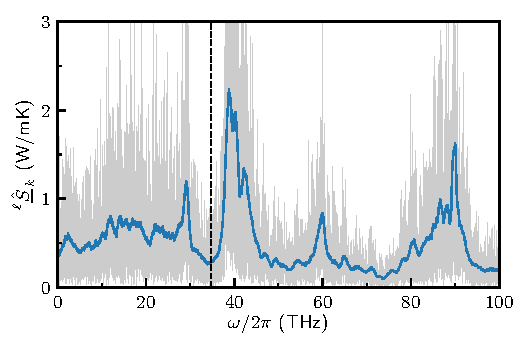
\includegraphics[width=8cm]{chapters/chapter5/figures/psd_water_ethanol_40.pdf}
    \caption{Multi-component power spectrum, as defined in Eq.~\eqref{eq:mean-multi-periodogram}, for a classical flexible model of a solution of water and ethanol $50\un{mol}\%$, obtained from a $100\un{ps}$ trajectory. Grey: $^{\ell}\hat{\underline{S}}_{\,k}$ obtained directly from Eq.~\eqref{eq:mean-multi-periodogram}, with $\ell=3$ and $Q=2$. Blue: $^{\ell}\hat{\underline{S}}_{\,k}$ filtered with a moving average window of width $1\un{THz}$ in order to reveal its main features. The vertical dashed line delimits the low-frequency region used in the subsequent cepstral analysis. Reproduced from Ref.~\cite{Bertossa2018}.
    }
    \label{fig:grappa-periodogram}
\end{figure}

\begin{figure}[!tb]
    \begin{center}
        \subfigure[]{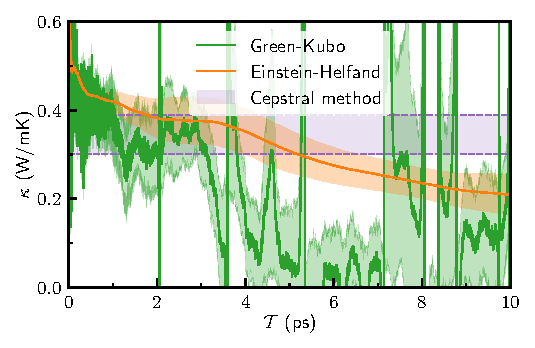
\includegraphics[width=6.8cm]{chapters/chapter5/figures/gk-grappa_capitolo_40.pdf}}
        \hfill
        \subfigure[]{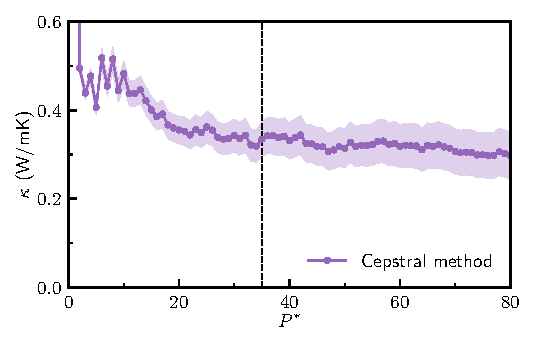
\includegraphics[width=6.8cm]{chapters/chapter5/figures/convergence_water_ethanol_40.pdf}}
    \end{center}
	\caption{Convergence of the multi-component thermal conductivity estimator $\kappa$ using the direct time-integration approach and the cepstral method, for a classical flexible model of a solution of water and ethanol $50\un{mol}\%$, obtained from a $100\un{ps}$ trajectory.
    (a) Direct time-integration approach in its Green-Kubo (green, as obtained from the matrix $L^{ij}(\mathcal{T})\propto\int_0^\mathcal{T} \left\langle J^i(t) J^j(0) \right\rangle dt $) and Einstein-Helfand (orange -- obtained from the  matrix $\left (L^{ij}\right )'(\mathcal{T}) \propto  \int_0^\mathcal{T}\left(1-\frac{t}{\mathcal{T}}\right) \left \langle J^i(t) J^j(0) \right \rangle dt$) formulations. The horizontal purple band indicates the value obtained by the cepstral method.
    (b) Estimate of $\kappa$ with the cepstral method as a function of the number of cepstral coefficients, $P^*$, see Eqs.~(\ref{eq:L0*}-\ref{eq:sigma*}). The dashed vertical line indicates the value of $P^*$ selected by the AIC, Eq.~\eqref{eq:AIC-P}. Reproduced from Ref.~\cite{Bertossa2018}.
    }
    \label{fig:twoCompConvergence}
\end{figure}


\subsection{Discussion}
The method discussed so far shows a fundamental advantage with respect to a na\"ive implementation of direct time-integration approach.
Fig.~\ref{fig:twoCompConvergence} shows the two-component conductivity $\kappa$, obtained via Eq.~\eqref{eq:kappa-integralT} as a function of the upper time-integration limit $\mathcal{T}$, 
\begin{equation}
    \kappa(\mathcal{T}) = \frac{1}{T^2} \left( L^{\smallE\smallE}(\mathcal{T}) - \frac{(L^{\smallE\smallQ}(\mathcal{T}))^2}{L^{\smallQ\smallQ}(\mathcal{T})} \right),  \label{eq:two-comp-kappa-integralT}
\end{equation}
in the case of a water-ethanol solution. Both the Green-Kubo and the Einstein-Helfand definitions of the finite-time expression of Onsager's coefficients (see Eq.~\eqref{eq:Einstein-Helfand-Lij}) are displayed.
Due to thermal fluctuations, the integral of the correlation function becomes a random walk as soon as the latter vanishes, eventually assuming any value. Therefore, there will be a set of times (see Fig.~\ref{fig:twoCompConvergence}) where the term $L^{\smallQ\smallQ}$ at the denominator in Eq.~\eqref{eq:two-comp-kappa-integralT} vanishes, leading to divergences in the evaluation of $\kappa$; an issue not affecting the one-component case. Hence, in such a formulation of the multi-component case, the mean value of the thermal conductivity estimator \textit{in the time domain} does not exist. On the contrary, the multi-component frequency-domain approach presented in this section, and built on sound statistical basis, provides a well defined expression for the estimator of $\kappa$ and its statistical error.


\subsection{Data analysis work-flow (multi-component fluids)}  \label{sec:cepstral-workflow-multicomp}
We summarize the steps leading to the estimation of thermal conductivity by the \textit{cepstral analysis} method for multi-component fluids, in the same way we did in Sec.~\ref{sec:cepstral-workflow-1comp} for solids and one-component fluids. 
\begin{enumerate}
\item From a MD simulation compute the heat flux time series $J_n^1$ and the independent particle fluxes $J_n^q$, $q=2,\dots,Q$.
\item Compute the discrete Fourier transform of the fluxes, $\tilde{J}^{\small i}_k$, and the element $1/(\hat{S}^{-1})^{\smallone\smallone}$. In practice, only a selected low-frequency region shall be used (see \cite{Ercole2017} for a detailed discussion).\footnote{To lighten the notation, we drop the left superscripts of the variables in this subsection.}
\item Calculate $\log\left[1/(\hat{S}^{-1})^{\smallone\smallone}\right]$.
\item Compute the inverse discrete Fourier transform of the result to obtain the cepstral coefficients $\hat{C}_n$.
\item Apply the Akaike Information Criterion, Eq.~\eqref{eq:AIC-P}, to estimate the number of cepstral coefficients to retain, $P^*$.
\item Finally apply Eq.~\eqref{eq:L0*} to obtain $\hat{L}_0^*$, and evaluate the thermal conductivity as
\begin{equation}
\kappa = \frac{\rOmega}{2k_B T^2} \exp\left[\hat{L}_0^* - \psi(\ell - Q+1) + \log(\ell -Q+1) \right],
\end{equation}
and its statistical error as
\begin{equation}
\frac{\rDelta\kappa}{\kappa} = \sqrt{\psi'(\ell -Q+1) \frac{4P^{*}-2}{N}}.
\end{equation}
\end{enumerate}


\section{Outlook}  \label{sec:data-analysis-outlook}

\begin{LEtext}
Although a large variety of methods has been formulated in the literature, none of them seem to provide a sufficiently rigorous and accurate estimator of the thermal conductivity, that can be applied to different classes of materials and especially to disordered systems. 
The cepstral analysis method introduced in this chapter promises to be a very powerful tool to estimate the thermal conductivity, from relatively short MD runs, in a more rigorous way than done so far by other methods. 
Its implementation is straightforward and its use robust, as the only parameter to be determined is the optimal number of cepstral coefficients, using \emph{e.g.} the Akaike's information criterion.
The most impressive results are achieved for disordered systems, \emph{e.g.} liquids and amorphous solids, and multi-atom cells, where a low conductivity results from large cancellations in the integral of a highly oscillatory time auto-correlation function, where all the traditional methods fail or give very subjective results. In these systems, simulation times of the order of $100\un{ps}$ seem sufficient to obtain accuracies of the order of $10\%$ in the estimated thermal conductivities. 

The performance is less spectacular in periodic crystals, where slowly-decaying strongly-harmonic phonon modes require longer simulation times and the ensuing sharp peak in the low-frequency region of the power spectrum requires a larger number of cepstral coefficients than predicted by the optimization of the AIC. Even so, simulation times of the order of a few hundred picoseconds seem sufficient to achieve a comparable accuracy. In the latter case, it is possible that a combination of the methodology introduced here with specialized techniques based on normal-mode analysis, such as that presented in Ref.~\cite{Carbogno:2017gc}, will result in further improvements. 
Leveraging more general (possibly non-Fourier) representations of the log-spectrum of the currents to be analyzed, and replacing the optimization of the AIC with more sophisticated and possibly more efficient approaches, such as \emph{e.g.} weighted multi-model inference techniques \cite{Burnham2004,Claeskens2008}, may also assist in this and other difficult cases. 
Finally, we expect that our methodology will impact on the simulation of any transport phenomena to which the Green-Kubo theory applies, such as ionic conduction, viscosity, and many others: benchmarks on these properties should be performed. 

This achievement also overcomes the last hurdle towards the quantum simulation of heat transport, which has been considered out of its scope until very recently, due to the long trajectories usually required, and will be particularly important to study strongly anharmonic and/or disordered systems. 

\end{LEtext}
